\documentclass[11pt,letterpaper]{article}

\makeatletter
\renewcommand\paragraph{\@startsection{paragraph}{4}{\z@}%
                                      {1ex \@plus1ex \@minus.2ex}%
                                      {-1em}%
                                      {\normalfont\normalsize\bfseries}}
\makeatother

%%%%%%%%%%%%%%%%%%%%%
%  P A C K A G E S  %
%%%%%%%%%%%%%%%%%%%%%

% Authors
\usepackage{authblk}

% Page margins
\usepackage[margin=1in]{geometry}

% Nicer math font
\usepackage{mathpazo}

% More fancy lists
\usepackage{enumerate}

% Microtype
\usepackage{microtype}

% TikZ
\usepackage{tikz}
%\usetikzlibrary{calc,shapes.geometric}
\usetikzlibrary{backgrounds,fit,decorations.pathreplacing,calc}

% Highlights
\usepackage{soul}

% Young Tableaux
\usepackage{ytableau}

% Figure
\usepackage{float}

% Hypertext package
\usepackage[colorlinks = true]{hyperref}
% Title and authors
%\hypersetup{
%  pdftitle = {},
%  pdfauthor = {}
%}
% Color definitions
\definecolor{darkred}  {rgb}{0.5,0,0}
\definecolor{darkblue} {rgb}{0,0,0.5}
\definecolor{darkgreen}{rgb}{0,0.5,0}
% Color links
\hypersetup{
  urlcolor   = blue,         % color of external links
  linkcolor  = darkblue,     % color of internal links
  citecolor  = darkgreen,    % color of links to bibliography
  filecolor  = darkred       % color of file links
}

% AMS
\usepackage{amsmath,amssymb,amsfonts,amsthm,amstext}

%% Restating theorems
%\usepackage{thm-restate}

% Powerful macros
\usepackage{etoolbox}

% Fixes for amsmath
\usepackage{mathtools}
\mathtoolsset{centercolon}
\makeatletter
\protected\def\tikz@nonactivecolon{\ifmmode\mathrel{\mathop\ordinarycolon}\else:\fi}
\makeatother

% Daw boxes
\usepackage{tcolorbox}

% Code
\usepackage{algorithm}
%\usepackage{algorithmic}
\usepackage{algpseudocode}

% Clever references
\usepackage{cleveref}%[nameinlink]
\crefname{lemma}{Lemma}{Lemmas}
\crefname{proposition}{Proposition}{Propositions}
\crefname{definition}{Definition}{Definitions}
\crefname{theorem}{Theorem}{Theorems}
\crefname{conjecture}{Conjecture}{Conjectures}
\crefname{corollary}{Corollary}{Corollaries}
\crefname{claim}{Claim}{Claims}
\crefname{section}{Section}{Sections}
\crefname{appendix}{Appendix}{Appendices}
\crefname{figure}{Fig.}{Figs.}
\crefname{table}{Table}{Tables}
% \crefname{algorithm}{Algorithm}{Algorithms}

% IEEE tools
\usepackage[retainorgcmds]{IEEEtrantools}

% table of contents
\usepackage{tocloft}

% Table with multi-row
\usepackage{multirow}

% TikZ
\usepackage{tikz}	
\usetikzlibrary{backgrounds,fit,decorations.pathreplacing}

%%%%%%%%%%%%%%%%%%%%%%%%%
%  N E W C O M M A N D  %
%%%%%%%%%%%%%%%%%%%%%%%%%

% Standard quantum notation

\newcommand{\ket}[1]{|#1\rangle}
\newcommand{\bra}[1]{\langle#1|}
\newcommand{\braket}[2]{\langle#1|#2\rangle}
\newcommand{\ketbra}[2]{|#1\rangle\langle#2|}
\newcommand{\proj}[1]{|#1\rangle\langle#1|}

\newcommand{\x}{\otimes}
\newcommand{\xp}[1]{^{\otimes #1}}
\newcommand{\op}{\oplus}

\newcommand{\ct}{^{\dagger}}
\newcommand{\tp}{^\intercal}

% Linear algebra

%\newcommand{\1}{\mathbb{1}} % identity matrix
%\DeclareMathOperator{\Hom}{Hom}
\DeclareMathOperator{\End}{End}
%\DeclareMathOperator{\E}{\mathbb{E}}
\DeclareMathOperator{\Lin}{L} % all linear maps
\newcommand{\Mat}[1]{\mathrm{M}(#1)} % all matrices
%\newcommand{\Mat}[1]{\mathrm{M}_{#1}(\C)}

% Paired delimiters

\DeclarePairedDelimiter{\set}{\lbrace}{\rbrace}
\DeclarePairedDelimiter{\abs}{\lvert}{\rvert}
\DeclarePairedDelimiter{\norm}{\lVert}{\rVert}
\DeclarePairedDelimiter{\of}{\lparen}{\rparen}
\DeclarePairedDelimiter{\sof}{\lbrack}{\rbrack}
\DeclarePairedDelimiter{\ip}{\langle}{\rangle}
\DeclarePairedDelimiter{\floor}{\lfloor}{\rfloor}

% Operators

\renewcommand{\Re}{\operatorname{Re}}
\renewcommand{\Im}{\operatorname{Im}}
\DeclareMathOperator{\vc}{vec}
\DeclareMathOperator{\spn}{span}
\DeclareMathOperator{\rank}{rank}
\DeclareMathOperator{\diag}{diag}
\DeclareMathOperator{\spec}{spec}
\DeclareMathOperator{\Tr}{Tr}
\DeclareMathOperator{\sgn}{sgn}
\DeclareMathOperator{\hook}{hook}
\DeclareMathOperator{\E}{\mathbb{E}}
\DeclareMathOperator{\supp}{supp}


% Sets

\newcommand{\C}{\mathbb{C}}
\newcommand{\R}{\mathbb{R}}
\newcommand{\N}{\mathbb{N}}
\newcommand{\Z}{\mathbb{Z}}
\newcommand{\calH}{\mathcal{H}}
\newcommand{\calX}{\mathcal{X}}
\newcommand{\calY}{\mathcal{Y}}
\newcommand{\calA}{\mathcal{A}}
\newcommand{\calB}{\mathcal{B}}

% Group
\newcommand{\Zd}{\Z_d^{\times}}


% Identity operator
\newcommand{\1}{\mathbb{1}}

% Pauli Group
\newcommand{\Pg}{\mathcal{P}}
\newcommand{\J}{\mathcal{J}}

% Special notation

\newcommand{\CHSH}{CHSH^{(d)}}
\newcommand{\MS}{MS}
\newcommand{\SVT}{SVT}
\newcommand{\EPR}[1]{EPR^{(#1)}}
\newcommand{\paulix}{\sigma_x}
\newcommand{\pauliz}{\sigma_z}
\newcommand{\G}{G}
\newcommand{\LS}{LS}
\newcommand{\tA}{\tilde{A}}
\newcommand{\tB}{\tilde{B}}
\newcommand{\tX}{\tilde{X}}
\newcommand{\tZ}{\tilde{Z}}
\newcommand{\tU}{\tilde{U}}
\newcommand{\tW}{\tilde{W}}
\newcommand{\tx}{\tilde{x}}
\newcommand{\tpsi}{\tilde{\psi}}
\newcommand{\tri}{\Delta}
\newcommand{\lB}{\overline{B}}
\newcommand{\dr}[1]{d^{(#1)}}


% Probabilities
\newcommand{\pr}[2]{P(#1|#2)}
\newcommand{\pa}[2]{P_A(#1|#2)}
\newcommand{\pb}[2]{P_B(#1|#2)}

% Bell Ineqaulities
\newcommand{\I}{\mathcal{I}}


% Comments
\def\carl#1{{\color{blue} #1 -Carl}}
\newcommand{\hf}[1]{\textcolor{red}{#1}}

%%%%%%%%%%%%%%%%%%%%%%%%%
%  N E W T H E O R E M  %
%%%%%%%%%%%%%%%%%%%%%%%%%

\newtheorem{theorem}{Theorem}
\newtheorem{lemma}[theorem]{Lemma}
\newtheorem{proposition}[theorem]{Proposition}
\newtheorem{definition}[theorem]{Definition}
\newtheorem{corollary}[theorem]{Corollary}
\newtheorem{conjecture}[theorem]{Conjecture}
\newtheorem{claim}[theorem]{Claim}
\newtheorem*{conjecture*}{Conjecture}
\newtheorem*{problem}{Problem}
\newtheorem*{example}{Example}

\theoremstyle{definition}
\newtheorem*{remark}{Remark}



%%%%%%%%%%%%%%%%
%   Document   %
%%%%%%%%%%%%%%%%

\begin{document}

\title{Self-test prime dimensional EPR pairs with constant alphabet}

\author[1]{Honghao Fu}
\author[1,2]{Carl Miller}

\renewcommand\Affilfont{\itshape\small}



\affil[1]{Department of Computer Science, Institute for Advanced Computer Studies, and Joint Center for Quantum \break Information and Computer Science, University of Maryland, College Park, MD 20742, USA}
\affil[2]{National Institute of Standards and Technology, 100 Bureau Dr., Gaithersbug, MD 20899, USA}
\maketitle

%========================================
\section{Introduction}
\label{sec:intro}
%========================================
Self-testing is a unique phenomenon of quantum mechanics. It has many applications in quantum
delegated computation \cite{ruv2013,cgsv2017} and device independent quantum cryptography
\cite{qkd2011,qkd2014,miller2016,fu2018,eat2018}.

The case of self-testing $2$-dimensional EPR pair is fully understood. One can robustly self-test
one copy of it by the CHSH inequality \cite{bamps2015}. and self-test many copies of the $2$-dimensional EPR
pair in parallel \cite{mckague2016, coladan2017parallel}. 
Self-testing general $d$-dimensional EPR pairs is a harder task.
Recently, a remarkable result by Coladangelo \textit{et al}.\cite{cgs2017} 
has shown that the maximally entangled state with arbitrary local dimension 
can be self-tested with constant question alphabet but answer alphabet growing with
the local dimension. 
Then Coladangelo and Stark \cite{coladan2017} further showed that by playing many instances
of the generalized Magic Square game and Magic Pentagram game, one can robustly self-test
$N$ copies of the maximally entangled state with local dimension $d$ for any $d, N \geq 2$.
Both the Magic Square game and the Magic Pentagram game have constant question alphabet
but answer alphabet of size $d$.

At a high level, general $d$-dimensional maximally entangled states are self-tested by
modifying the correlation and enlarging the size of the correlation.
A natural question to ask is whether maximally entangled state with large local dimension
can be self-tested with fixed-sized correlation. 
An equivalent question to ask is whether it is possible to self-test maximally
entangled state of some local dimension more efficiently, with constant correlation size. 
In this report, we give an affirmative answer to this question by proving the following theorem.
\begin{theorem}[Informal]
\label{thm:inf}
	There exists an infinite-sized set $D$ of odd prime numbers such that, for any $d \in D$, 
	the maximally entangled state of local dimension $d-1$ can be self-tested 
	with constant-sized question and answer alphabets.
\end{theorem}

The set $D$ is easily characterizable as it contains all the odd prime numbers with smallest
primitive root $2$, $3$ or $5$. It has been shown that there are infinitely many prime numbers
with smallest primitive root in the set $\{2,3,5\}$ \cite{murty1988}, so the set $D$ has infinitely many elements.
To prove \cref{thm:inf}, we give explicit self-testing proof of 
the maximally entangled state with local dimension $d-1$ where the primitive root of $d$ is $2$,$3$, or $5$, 
by explicitly giving the correlation that achieves self-testing. 
%Then the self-testing property of this correlation is 
%given in the following theorem.
%\begin{theorem}[Informal]
%\label{thm:pr_2}
%	All maximally entangled state with local dimension $d-1$, where $d$ is prime and has
%	primitive root $r \in \{2, 3, 5\}$, can be self-tested by a constant-sized correlation.
%\end{theorem}
Our correlation is denoted by $C(\dr{r})$ for prime $d$.
We use the superscript $(r)$ to denote the primitive root of $d$.
Note that although the size of $C(\dr{r})$ does not depend on $d$, the optimal correlation does.


In order to accomplish our goal, we introduce new techniques for self-testing.
First of all, we use a different variant of the weighted CHSH inequality to enforce the eigenvalue of
some unknown operator which is the product of two binary observables used in the weighted CHSH test.
\carl{I think this game might have been defined in APM12, and if so we need to cite it.}
The variant of the CHSH inequality that we use is not used in the self-testing literature before.
Secondly, we give a new way to decompose unitaries of arbitrary order into binary observables which maintains
certain commutation relations. Such decomposition is different from what Slofstra used in his work \cite{slofstra2017}.
\carl{Our work is heavily based on \cite{slofstra2017}, and we need to make that clearer.}
Intuitively, such decomposition can be seen as the inverse of the Jordan's lemma decomposition.
The third contribution is that we prove self-testing without using anti-commutation relations between Pauli operators, 
which is the core idea in all the previous self-testing results.
\carl{Are we sure about that ("all")?}
Instead, we find a new pair of operators that can generate the ring of matrices over complex numbers.


\textbf{Structure of the paper}.
We start with notations and background information in \cref{sec:prelim}.
Since the correlation we designed can win a special linear system game and satisfy
an extended weighted CHSH test, we introduce the linear system game
in \cref{sec:lsg} and the extended weighted CHSH test in \cref{sec:chsh}. 
Our main result is based on the combination of the two tests and presented in \cref{sec:main}. 

%========================================
\section{Preliminaries and notations}
\label{sec:prelim}
%========================================
We use $[n]$ to denote the set $\{0,1 \dots n-1\}$ and $[n]+1$ for the set $\{1,2 \dots n\}$.
%We denote the group commutator of $A$ and $B$, i.e. $ABA^{-1}B^{-1}$, by $[A,B]$.

We use some basic number theory in our work. A primitive root of a prime number
$d$ is an integer $r$ such that $r \pmod{d}$ has multiplicative order $d-1$. Equivalently,
$r$ is the generator of the multiplicative group of integers modulo $d$, $\Zd$ where
$\Zd = \{1,2\dots d-1\}$. \textcolor{red}{When the prime number $d$ has multiple primitive roots,
we always work with the smallest one.}
\carl{I'm not clear on what that last sentence means.  You just defined what a primitive root
is --- are you changing the definition now?}

The EPR pair of local dimension $d-1$ for some prime $d$ is denoted by
\begin{align}
\ket{\EPR{d-1}} = \frac{1}{\sqrt{d-1}} \sum_{i = 0}^{d-2} \ket{ii}.
\end{align}
The superscript $(d-1)$ stresses the local dimension and we follow this convention through this paper.

We self-test $\ket{\EPR{d-1}}$ by verify that Alice and Bob has operators
\begin{align}
	X = \sum_{k=1}^{d-1} \omega_d^k\ketbra{k}{k} && U = \sum_{k=1}^{d-1} \ketbra{k/r}{k},
\end{align}
where $\omega_d = e^{i2\pi/d}$ is the primitive $d$-th root of unity,
and $r$ is the primitive root of $d$.  \carl{That sentence is jumping ahead --- you should just stick to
definitions and notation for now.}
Through out this paper, any operation on the label of the eigenvector $\ket{k}$ is taken modulo $d$,
unless otherwise specified, for example, the $k/r$ above.

\textbf{The weighted CHSH inequality \cite{acin2012}.}
The first building-block of our result is a robust self-testing result based on the weighted CHSH inequality.
In the CHSH scenario, Alice and Bob has binary observables $A_x,B_y$ for $x,y = 1,2$ 
on Hilbert space $\calH_A$ and $\calH_B$ respectively.  \carl{It needs to be clearer who Alice and Bob
are --- perhaps you should put this subsection after the ``Nonlocal games'' subsection.}
A binary observable is a Hermitian matrix whose only eigenvalues are either $+1$ or $-1$.
The weighted CHSH inequality is given by 
\begin{align}
	\label{eq:chsh_op}
	\I_\alpha = \alpha\ip{A_1B_1}+\alpha\ip{A_1B_2} + \ip{A_2B_1} - \ip{A_2B_2}\leq 2\alpha,
\end{align}
where $\ip{A_xB_y}$ is the expectation value of of the observables.  \carl{Same here -- it's not clear enough
what this means until the reader has seen the ``Nonlocal games'' subsection.}
If Alice and Bob share product state $\ket{\phi} = \ket{\phi_A} \x \ket{\phi_B}$, they cannot violate
the weighted CHSH inequality.
However, If they share entangled state $\ket{\psi}$, the maximal violation is 
\begin{align}
\label{eq:chsh_max}
 \I_\alpha \leq 2\sqrt{1+\alpha^2}.
\end{align}
\begin{definition}[Ideal strategy for $\I_\alpha$]
	\label{def:ideal}
	Define $\mu = \arctan(1/\alpha)$.
	The ideal strategy for weighted CHSH with parameter $\alpha$ (i.e. achieving maximal violation in \cref{eq:chsh_max})
	consists of the joint state $\ket{\EPR{2}}$ and observables $A_1 = \pauliz$, $A_2 = \paulix$,
	$B_1 = \cos(\mu) \pauliz+ \sin(\mu) \paulix$ and $B_2 = \cos(\mu) \pauliz - \sin(\mu) \paulix$.
\end{definition}
\carl{Just to be complete, you should say what $\pauliz$ and $\paulix$ denote.}
An interesting observation of the weighted CHSH inequality is that its maximal violation can certify the shared states and the 
measurements up to isometry, 
which is a phenomenon referred as a self-test. We give formal statement of this self-testing result in \cref{sec:chsh}.

\textbf{Nonlocal games}. The two players of a nonlocal game are Alice and Bob. Each of them is requested
to give an answer for a randomly chosen question. We denote Alice's question set by $\calX$ and answer set by $\calA$. Similarly,
Bob's question set is denoted by $\calY$ and his answer set is denoted by $\calB$. The nonlocal game also
comes with two functions: $\pi: \calX \times \calY \rightarrow [0,1]$, which is the probability distribution over the questions,
and $V: \calA \times \calB \times \calX \times \calY \rightarrow \R$, which is the scoring function. Such games are nonlocal
because Alice and Bob cannot communicate after getting their questions but they may share some strategy before 
the start of the game. Note that in the literature, the typical scoring function of a nonlocal game maps the input-output
pair to $\{0,1\}$ which corresponds to losing and winning. Allowing the score to be any real number is the key ingredient 
to our new result. 

A quantum strategy of a game $G$ consists of projective measurements $\{\{A_x^a\}_a\}$ on Alice's side, 
$\{\{B_y^b\}_b\}_y$ on Bob's side, and a shared state $\ket{\psi}$, where a projective measurement $P$ satisfies
the condition that $P^2 = P = P\ct$.  \carl{You need to put explicit labels on the quantum systems used by
Alice and Bob.  (Later on you seem to use ``$A$'' and ``$B$'' to refer to those systems, but those are also
the same letters you use for Alice's and Bob's measurements.  That's confusing.)}
Then Alice and Bob's quantum strategy produces the correlation
\begin{align}
	\pr{ab}{xy} = \bra{\psi} A_x^a \x B_y^b \ket{\psi} \text{ for all } (a,b,x,y) \in \calA \times \calB \times \calX \times \calY,
\end{align}
where $(A_x^a)^2 = A_x^a = (A_x^a)^\dagger$ and $(B_y^b)^2 = B_y^b = (B_y^b)^\dagger$.
%Note that we may use the term behaviour and correlation interchangeably.
%The value of a strategy is given by
%\begin{align}
%	\omega(G,p)  = \sum_{a,b,x,y} \pi(x,y) \pr{ab}{xy} V(a,b,x,y).
%\end{align} 

The main contribution of our work is the construction of a correlation, which is the combination of 
the optimal correlation of a linear system game with constant-sized $\calX$,$\calY$,$\calA$ and $\calB$
and the optimal correlation to violate the weighted CHSH inequality.  \carl{The reader does not 
know yet what a linear system game is, so this comment is more confusing than helpful.}
The special property of the correlation is that it can self-test $\ket{\EPR{d-1}}$ for arbitrary $d$ with certain 
primitive root. 
In the next part, we introduce the definition of self-testing, the definition of linear system game, 
and its operator solution, 
following definitions given in Ref.~\cite{coladan2017, slofstra2017}.

\carl{Before the next definition, you should define what a ``correlation'' is.}
\begin{definition}[Self-testing]
	We say that a correlation self-tests a quantum state $\ket{\psi}$, if 
	the correlation is produced by a strategy with shared state $\ket{\psi}$, and 
	for any quantum strategy $S = ( \{\tA_x\}, \{\tB_y\}, \ket{\tpsi})$ that produces the same correlation,
	there exists local isometries $\Phi_A$ and $\Phi_B$ on Alice and Bob's side and a state $\ket{junk}$ 
	such that 	
	\begin{align*}
		\Phi_A \x \Phi_B \ket{\tpsi} =  \ket{\psi} \x \ket{junk}.
	\end{align*}
\end{definition}
\begin{definition}[Linear system game]
 Let $Hx = c$ be an $m \times n$ system of linear equations over $\Z_2$,
 where $H$ is an $m$-by-$n$ matrix with entries in $\Z_2 = \{0,1\}$ and 
 $c$ is a length-$n$ vector with entries in $\Z_2$. 
 The associated linear system game involves two
 players Alice and Bob, where Alice is given an equation number $i \in \calX = [m]+1$ and replies with $a \in \calA = \Z_2^{\times n}$,
 and Bob is given a variable number $j \in \calY = [n]+1$ and replies with an assignment $b \in \calB = \Z_2$. The winning condition is 
 that Alice's assignment to the variables should satisfy equation $i$ and Alice's $j$-th assignment $a(j)$ should match $b$.
 Formally, the winning condition is 
 \begin{align*}
 	a(j) &= b && \text{(Consistency)} \\
	\sum_{k= 1}^n H(i,k) a(k) &\equiv c(i) \pmod 2. &&\text{(Constraint satisfaction)},
 \end{align*}
 for all $(i,j) \in \calX \times \calY$. 
\end{definition}
The scoring function of linear system games always maps an input-output pair to $\{0,1\}$, 
so later when we say a quantum strategy wins a linear system game perfectly, we mean that 
$V(a,b,x,y) =0$ implies that $\pr{ab}{xy} = 0$.  \carl{Make this clear in the definition itself.}
We focus on quantum strategies for the linear system game presented in terms of binary observables.
\begin{definition}[Quantum strategy of a linear system game]
\label{def:q_strat}
A quantum strategy for the linear system game $(Hx = c)$ consists of 
\begin{enumerate}
	\item a pair of finite Hilbert spaces $\calH_A$ and $\calH_B$;
	\item a collection of binary observables $B_j$, $1 \leq j \leq n$, on $\calH_B$
	such that $B_j^2 = \1$ for every $1 \leq j \leq n$;
	\item a collection of binary observables $A_{ij}$, $1\leq i \leq m$, $1\leq j\leq n$ 
	on $\calH_A$ such that 
	\begin{enumerate}
		\item $A_{ij}^2 = \1$ for every $i,j$,
		\item $\Pi_j A_{ij}^{H(i,j)} = (-\1)^{c(i)}$ for every $i$, and
		\item $A_{il}A_{ik} = A_{ik}A_{il}$ for every $i$ and $H(i,l) = H(i,k) =1$;
	\end{enumerate} 
	and
	\item a quantum state $\ket{\psi} \in \calH_A \x \calH_B$.
\end{enumerate}
\end{definition}
Note that any quantum strategy presented in terms of binary observables can be 
converted to a quantum strategy presented in terms of projective measurement, and
vice versa.  \carl{This is not entirely true.  A ``quantum strategy presented in terms of projective measurement'' allows
Alice to give answers that violate the ``Constraint satisfaction'' condition, while a ``quantum strategy presented 
in terms of binary observables'' does not.}

It has been shown in Ref.~\cite{cleve2014} that the linear system game has a perfect strategy 
satisfying conditions in \cref{def:q_strat} if and only if the linear system has a finite-dimensional
operator solution in the following sense.  \carl{There's a missing reference here?}
\begin{definition}[Operator solution of a linear system]
\label{def:op_sol}
	An operator solution to a linear system $Hx =c$ over $\Z_2$ is a sequence of bounded Hermitian 
	operators $A_1, A_2, \dots A_n$ on a Hilbert space $\calH$ such that \carl{(What does the word ``bounded'' mean here?  It might
	be best to just state the definition for finite dimensions only.)}
	\begin{enumerate}
		\item $A_i^2 = \1$, i.e. $A_i$ is a binary observable, for all $1 \leq i \leq n$;
		\item If $x_l$ and $x_k$ appear in the same equation, then $A_l$ and $A_k$ commute;
		\item for all $1 \leq i \leq m$,
		\begin{align*}
			\Pi_{k=1}^n A_k^{H(i,k)} = (-1)^{c(i)}\1.
		\end{align*}
	\end{enumerate}
	A finite dimensional operator solution to a linear system $Hx = c$ over $\Z_2$ is an operator
	solution in which the Hilbert space is finite-dimensional.
\end{definition}
Perfect quantum strategies can be extracted from operator solutions and vice versa.
Another angle to look at the linear system game ($Hx = c$) is a finitely presented group
over $\Z_2$, which is called the solution group.
\begin{definition}[Solution group of a linear system game]
	\label{def:presentation}
	Let $Hx = c$ be an $m \times n$  linear system. The solution group of this system
	is the group
	\begin{align*}
		\Gamma(H,c) := \ip{
		x_1,\dots x_n, J: &J^2 = x_i^2 = e \text{ for all }1 \leq i \leq n, \\
				& \Pi_{j=1}^n x_j^{H(i,j)} = J^{c(i)} \text{ for all } 1 \leq i \leq m, \text{ and } \\
				& x_l x_k = x_k x_l \text{ if } H(i,k) = H(i,l) = 1 \text{ for some } i
				} .
	\end{align*}
\end{definition}
\carl{Don't you also need a commutativity condition for $J$ with $\{ x_i \}$?}
For concepts about group presentations, we refer to Sec.~$2$ of Ref.~\cite{slofstra2017}.
Combining \cref{def:op_sol} and \cref{def:presentation}, we know that an operator solution associated to $Hx =c$ is 
a finite-dimensional representation of $\Gamma(H,c)$ that maps $J$ to $-\1$.

\carl{Section 2 needs to be cleaned up in some places, but overall it is pretty good.}


%The main tool to understand linear system game is through its solution group over $\Z_d$.
%\begin{definition}[Solution group over $\Z_d$ \cite{coladan2017}]
%	For the linear system game associated with $Ax = b$ over $\Z_d$, its solution group $\Gamma(A,b,\Z_d)$ has 
%	one generator for each variable and one relation for each equation and relations enforcing that the variables in the same
%	equation commutes. The set of local commutativity relations is denoted by $R_c$ and defined by
%	\begin{align}
%		R_c := \set{ [x_i, x_j] |  A_{li} \neq 0 \neq A_{lj} \text{ for some } 1 \leq l \leq m}.
%	\end{align}
%	The set of constraint satisfaction relations is denoted by $R_{eq}$ and defined by.
%	\begin{align}
%		R_{eq} := \set{ \J^{-b(l)} \Pi_{i=1}^n  x_i^{A_{li}} | 1\leq l\leq m}
%	\end{align}
%	Then the solution group has presentation 
%	\begin{align}
%	\Gamma(A,b,\Z_d) := \ip{ \{x_i\}_{i=1}^n \cup \{\J\} : R_c \cup R_{eq} \cup \{ (x_i)^d, \J^d| 1 \leq i \leq n\}}. 
%	\end{align}
%\end{definition}
%Note that the relations $(x_i)^d$ and $\J^d$ ensure that we have solutions over $\Z_d$.
%Then the operator solution of $\Gamma(A,b,\Z_d)$ is given below.
%\begin{definition}[Operator solution]
%	An operator solution for the linear system game associated with $Ax =b$ over $\Z_d$ is a unitary representation
%	$\tau$ of $\Gamma(A,b,\Z_d)$ such that $\tau(\J) = \omega_d\1$. A conjugate operator solution is a unitary 
%	representation mapping $\J$ to $\overline{\omega_d}\1$.
%\end{definition}
%What has been established in Ref.\cite{cleve2017,coladan2017} is that we can construct a perfect strategy of a
%linear system game from its operator solution and vice versa.


%=======================================
\section{The linear system game}
\label{sec:lsg}
%=======================================
The goal of this section and the following two sections is to 
present a correlation that can self-test $\ket{\EPR{d-1}}$, 
where $d$ is prime and has primitive root $r \in \{2, 3, 5\}$,
and this correlation is denoted by $C(\dr{r})$.  \carl{Be more precise --- we are constructing
such a correlation for any $d$ which has $2, 3,$ or $5$ as a primitive root.}
The correlation we constructed is the optimal correlation for a game $\G(\dr{r})$, which is the combination of two tests.
In this section, we introduce the linear system game which tests a relation that should be satisfied by 
Alice and Bob's observables.

Slofstra's seminal work~\cite{slofstra2017} draws our attention to the relation $xyx^{-1} = y^2$.  \carl{That sentence
is too vague -- either make it a rigorous statement or leave it out.}
The main component of $\G(\dr{r})$ is a linear system game $\LS$, whose solution group is the embedding of the 
following group
\begin{align}
	\Pg_r= \langle u, x : uxu^{-1} = x^r \rangle, \text{ for } r \in \{2, 3,5\}.
\end{align}
In other words, relations in the presentation of the solution group of $\LS_r$ can be combined to derive the
relation $uxu^{-1} = x^r$.  
\begin{proposition}
	\label{prop:embed}
	The group $\Pg_r$ can be embedded into a linear system game $\LS_r$ over $\Z_2$,
	with constant numbers of variables and equations, where each equation involves $3$ variables.
	\carl{You need to make this a more precise statement.  (It sounds as if you're saying 
	that the numbers of variables and equations is independent of $r$, which I'm pretty sure is not true.)}
\end{proposition}
The process of embedding $\Pg_r$ into the solution group of $\LS$ follows the recipe given in the proofs of
Proposition~$4.8$, Lemma~$4.4$ and Proposition $4.2$ of Ref.~\cite{slofstra2017}.
The order of applying the results is the reverse of the order they are presented in Ref.~\cite{slofstra2017}.
We give details of this embedding process in \cref{sec:power2} for $r = 2$, \cref{sec:power3} for $r = 3$, 
and \cref{sec:power5} for $r = 5$. 

In the later parts of the paper, we use $n_r$ and $m_r$ to refer to the size of $\LS_r$.
The key feature of this embedding is that $\LS_r$ has constant-sized input-output alphabet
even if the generators $u$ and $x$ have arbitrary order. 
The product of the generators $x_1$ and $x_2$ from the solution group of $\LS_r$ plays the role 
of the generator $x$ in $\Pg_r$ and the product of the generators $x_3$ and $x_4$ plays the role
of the generator $u$ in $\Pg_r$.   \carl{It's reasonable to make a couple informal statements
at the beginning of a section, but you shouldn't be making
such vague statements at this point.  Everything said at this point in the section should have a precise mathematical
meaning.}
As shown in \cref{sec:power2}, \cref{sec:power3} and \cref{sec:power5}, 
$x_1$,$x_2$,$x_3$ and $x_4$ satisfy the relation
\begin{align}
	(x_3x_4)(x_1x_2)(x_4x_3) = (x_1x_2)^r.
\end{align}
Hence the perfect quantum strategy $(\ket{\psi}, \{A_i, B_i\}_{i=1}^n)$ should satisfy 
the key relation that 
\begin{align}
	(A_3A_4) (A_1A_2)(A_4A_3) \ket{\psi} = (A_1A_2)^r\ket{\psi}, 
\end{align}
and similarly on Bob's side.
If we denote the unitary corresponding to the generator $u$ of $\Pg_r$ by $U$ and the unitary
corresponding to $x$ by $X$, then $U = A_3A_4$, $X= A_1A_2$, and 
$UXU\ct \ket{\psi} = X^r \ket{\psi}$.
The special property of $U$ and $X$ is summarized in the following lemma. 

\begin{lemma}
	\label{lm:ux_independ}
	Suppose there exist unitaries $U$ and $X$ which have the following forms
	\begin{align}
		X = \sum_{i=1}^{d-1} \omega_d^i \ketbra{i}{i} && U = \sum_{i=1}^{d-1}\ketbra{i/r}{i},
	\end{align}
	where $d$ is an odd prime number with primitive root $r$,
	then the set $\{U^k X^l\}$ for $k=0,1\dots d-2$ and $l = 1,2\dots d-1$ forms a basis of 
	the ring of $(d-1)\times (d-1)$ matrices over $\C$.
\end{lemma}
Note that the unitaries $U$ and $X$ defined in the lemma above satisfy the condition $UXU^\dagger = X^r$.
In the self-test proof, this lemma will be a critical step.
\begin{proof}
We are going to show the $(d-1)^2$ matrices from the set $\{U^k X^l\}_{k \in[d-1], l \in [d-1]+1}$ are linearly independent.
Suppose there exists a set of complex numbers $\{ x_{k,l} \}_{k \in[d-1], l \in [d-1]+1}$
such that 
\begin{align}
	M = \sum_{k=0}^{d-2} \sum_{l=1}^{d-1} x_{k,l} U^k X^l = 0. 
\end{align}
We further assume that there exists a set of integers $\{ k_i \}_{i=1}^{d-1}$ such that $r^{k_i} \equiv i \pmod{d}$.
\carl{We shouldn't be making extra assumptions that are not stated in the lemma.  This looks to me more like
a definition of the variables $\{ k_i \}$, rather than an assumption.}
The fact that $r$ is a primitive root of $d$ guarantees that $k_i$'s are distinct.
Then we can group $\{x_{k,l}\}$ into vectors: $\ket{x_{k_1}}, \ket{x_{k_2}} \dots \ket{x_{k_{d-1}}}$,
where $\ket{x_{k_i}}= (x_{k_i, 1}, x_{k_i, 2} \dots x_{k_i, d-1})^\intercal$.
Our goal is equivalent to proving that $\ket{x_{k_i}} = 0$ for all $i$.

We start with proving that $\ket{x_{k_1}} = 0$.
Proving $\ket{x_{k_i}} = 0$ for other $i$ follows a similar argument, so we briefly
discuss about it in the end.
The entry $\bra{1}M\ket{1}$ can be expressed as  
\begin{align}
	\bra{1}M\ket{1} = \sum_{k=0}^{d-2}\sum_{l = 1}^{d-1}\sum_{i=1}^{d-1} x_{k, l}\omega_d^{il}\braket{1}{i/r^k}\braket{i}{1}.
\end{align}
For the term $\braket{1}{i/r^k}\braket{i}{1} \neq 0$ we must have $i = 1$ and $r^k \equiv 1 \pmod{d}$, or equivalently,
$k = k_1$. We can conclude that 
\begin{align}
	\bra{1}M\ket{1} = \sum_{l = 1}^{d-1} x_{k_1,l}\omega_d^l = 0. 
\end{align}
Similarly we can determine that for all $j = 1,2\dots d-1$,
\begin{align}
	\bra{j}M\ket{j} 
	=  \sum_{k=0}^{d-2}\sum_{l = 1}^{d-1}\sum_{i=1}^{d-1} x_{k, l}\omega_d^{il}\braket{j}{i/r^k}\braket{i}{j} 
	= \sum_{l = 1}^{d-1}x_{k_1,l}\omega_d^{jl} = 0.
\end{align}
Hence we get $d-1$ equations with $d-1$ variables, and the linear system is
\begin{align}
	W \ket{x_{k_1}} = 0,
\end{align}
where $W(m,n) = \omega_d^{mn}$. Then we define
\begin{align}
	\tW = 
	\begin{pmatrix}
	1 & 1 \\
	1 & W
	\end{pmatrix}.
\end{align}
First observe that $\tW$ is a Vandermonde matrix, hence it is non-singular.
Next, we define $\ket{\tx_{k_1}} = (0, x_{k_1,1}, \dots x_{k_1,d-1})^\intercal$ 
and prove that it satisfies the condition
that 
\begin{align}
	\tW \ket{\tx_{k_1}} = 0,
\end{align}
which involves $d$ equations. The last $d-1$ equations are given by the assumption and $M$.
We only need to prove that $\sum_{l=1}^d x_{k_1, l} = 0$, which is required by the first row of $\tW$.
It can be proved by summing the known $d-1$ equations as follows
\begin{align}
	0=\sum_{j = 1}^{d-1} \bra{j}M\ket{j}  
	=  \sum_{j=1}^{d-1}\sum_{l = 1}^{d-1}x_{k_1,l}\omega_d^{jl}
	=\sum_{l = 1}^{d-1}x_{k_1,l} (\sum_{j=1}^{d-1} \omega_d^{jl})
	= \sum_{l = 1}^{d-1}- x_{k_1,l}
\end{align}
where we have used the fact that $\sum_{j=1}^{d-1} \omega_d^{jl} =-1$ for all $l = 1,2\dots d-1$.
Since $\tW$ is non-singluar, we know $\ket{\tx_{k_1}} = 0$ which implies that $\ket{x_{k_1}} = 0$.

For $\ket{x_{k_a}}$, we look at entries $\{\bra{j}M\ket{aj}\}_{j=1}^{d-1}$ for $a = 2 \dots d-1$ and get equations
of the form
\begin{align}
	0 = \bra{j}M\ket{aj} = \sum_{l=1}^{d-1} x_{k_a, l} \omega_d^{ajl} 
\end{align}
The corresponding coefficient matrix has value $\omega_d^{amn}$ at coordinate $(m,n)$,
so it is also a submatrix of a Vandermonde matrix. Similar argument gives us that $\ket{x_{k_a}} = 0$.

To summarize, we have proven that $x_{k,l} = 0$ for all $k$ and $l$, which implies that the elements of the set
$\{ U^k X^l \}$ are linearly independent and forms a basis for the ring of all the $(d-1)\times(d-1)$ matrices over $\C$.
\carl{Nice proof.  I like the use of the Vandermonde matrix.  We can think a little about possible simplifications.}
\end{proof}
Note that the primitive root $r$ in the lemma is not restricted to the set $\{2,3,5\}$, so this lemma works for any 
odd prime number $d$.

%\begin{align}
%	\Pg_d = \langle x, z, \J : x^d = z^d = \J^d = e, zxz^{-1}x^{-1} = \J, x\J x^{-1}\J^{-1}= z\J z^{-1}\J^{-1} = e\rangle. 
%\end{align}
%The goal of our modification is to construct $\Pg_{\LS}$ which has implicit $d$-dependence.
%We first introduce new generators $u_x$ and $u_z$ to $\Pg_d$, and replace the relation $x^d = z^d = e$ 
%by the following relations
%\begin{align}
%\label{eq:sim}
%	u_x x u_x = x^2, \quad
%	u_z z u_z = z^2.
%\end{align}
%Consequently, the $d$ dependency of $\G$ comes from constraints imposed by other components of the game,
%\footnote{Figuring out what $a$ is will take us one step closer to resolving Artin's Conjecture\cite{murty1988}.}
%but the alphabet sizes are determined by $\Pg_{\LS}$ and we will see why they are constant.
%Next, we drop the relation $\J^d = e$ and make the value of $\J$ determined by $x$ and $z$ in the 
%relation $xzx^{-1}z^{-1} = \J$.
%
%It can be easily checked that $\paulix{d}$ and $\pauliz{d}$ can be extended to a representation of $\Pg_{\LS}$ 
%where  $\paulix{d}$ and $\pauliz{d}$ are defined by
%\begin{align}
%	\paulix{d} = \sum_{i=0}^{d-1} \ketbra{i+1 \pmod{d} }{i}  \quad \quad
%	\pauliz{d} = \sum_{i=0}^{d-1} \omega_d^i \ketbra{i}{i}.
%\end{align}
%Moreover, if $U_x\paulix{d}U_x^\dagger = (\paulix{d})^2$ and $U_z\pauliz{d}U_z^\dagger = (\pauliz{d})^2$,
%we can verify that 
%\begin{align}
%	U_xU_z = \1 = U_zU_x,
%\end{align}
%Hence, we do not need both $u_x$ and $u_z$ as generators and we just need one of them.
%In the end, we define $\Pg_{\LS}$ by
%\begin{equation}
%\begin{aligned}
%	\Pg_{\LS} =  \langle x, z, u, \J :  &zxz^{-1}x^{-1} = \J, [x,\J]=[z,\J]=[u,\J] = e, \\
%	&uxu^{-1} = x^2, u^{-1}zu = z^2 \rangle. 
%\end{aligned}
%\end{equation}
%This group will be embedded in a solution group, $\Gamma(\LS)$, following Slofstra's embedding techniques.
%The corresponding game $\LS$ has $n = 2351$ variables and $m= 1916$ equations.

%======================================
\section{The extended weighted CHSH test}
\label{sec:chsh}
%======================================
Before introducing the extended weighted CHSH test, we fill in some background about the weighted CHSH inequality,
namely, that its maximal violation can self-test $2$-dimensional EPR pair and rotated Pauli operators.
The robust self-testing result is summarized in the following theorem.
\begin{theorem}
\label{thm:selftest}
	Suppose the quantum strategy $(\ket{\tpsi}, \{\tilde{A}_x\}_{x \in [2]+1}, \{\tilde{B}_y\}_{y \in [2]+1})$ achieves the violation
	at least $2\sqrt{1+\alpha^2} - \epsilon$
	for some $\epsilon$, then
	there exists a local isometry $\Phi = \Phi_A \x \Phi_B$ and an auxiliary state $\ket{aux}$  such that
	\begin{align}
		\| \Phi( \tilde{A}_x \x \tilde{B}_y \ket{\psi}) -\ket{junk} \x (A_x \x B_y) \ket{\EPR{2}}  \| = O((\alpha^2+\frac{1}{\alpha}) \sqrt{\epsilon})
	\end{align}
	for $x,y \in \{0, 1, 2\}$ where the subscript $0$ refers to the identity operator and $A_x, B_y$ are 
	defined in \cref{def:ideal}.  \carl{You're using both ``aux'' and ``junk'' for the auxilliary state.  Also you need
	to be clearer about what label you are using for Alice's and Bob's systems (see my previous comment on this).}
\end{theorem}
Our approach is very similar to the one used in Ref.~\cite{bamps2015} so we 
defer the proof of \cref{thm:selftest} till \cref{sec:selftest}.
After proving the robust self-testing result, we take one step further and observe an interesting property of the 
product of Bob's observables.
\begin{proposition}
\label{prop:2d-subspace}
	Let $\mu = \arctan(1/\alpha)$ for some $\alpha$.
	If a quantum strategy $(\ket{\tpsi}, \{\tilde{A}_x\}_{x \in [2]+1}, \{\tilde{B}_y\}_{y \in [2]+1})$ achieves the maximal 
	violation of  $\I_{\alpha}$, then \hf{the only eigenvalues of $\tilde{B}_0\tilde{B}_1$ on the support of 
	$\tilde{\rho}_B = \Tr_A(\ketbra{\tpsi}{\tpsi})$
	are $e^{i2\mu}$ and $e^{-i2\mu}$.}  \carl{Make clear
	that we mean that these are the only eigenvalues.}
\end{proposition}
\begin{proof}[Proof of \cref{prop:2d-subspace}]
	Following the argument in the proof of \cref{thm:selftest} in \cref{sec:selftest}, we define
	\begin{align*}	
	\tilde{Z}_A = \tA_1, &&
	\tilde{Z}_B = (\tB_1+\tB_2)/2\cos(\mu).
	\end{align*}
	Substituting $\epsilon = 0$ into \cref{eq:zazb} we know that 
	\begin{align}
		\tZ_B \ket{\tpsi} = \tZ_A \ket{\psi}.
	\end{align}
	Using this relation, we get
	\begin{align}
		\tZ_B^2\ket{\tpsi} = \tZ_B \tZ_A\ket{\tpsi} = \tZ_A \tZ_B \ket{\tpsi} = \tZ_A^2 \ket{\tpsi} = \ket{\tpsi},
	\end{align}
	where we also use the facts that $\tZ_A$ and $\tZ_B$ commute and $\tZ_A^2 = A_1^2 = \1$.
	Hence we can conclude that $\tZ_B^2 =\1$ on $\supp(\tilde{\rho}_B)$.
	Expanding $\tilde{Z}_B^2$ we get
	\begin{align*}
		\1 = \tilde{Z}_B^2 = \frac{\tB_1^2 + \tB_1\tB_2 + \tB_2\tB_1 + \tB_2^2}{4\cos(\mu)^2}
		=\frac{2\1 + \tB_1\tB_2 + \tB_2\tB_1}{4\cos^2(\mu)},
	\end{align*}
	so we can derive that 
	\begin{align}
	\label{eq:eig_v}
		\tB_1\tB_2 + \tB_2\tB_1 = 2(2\cos^2(\mu)-1)\1 = 2 \cos(2\mu) \1.
	\end{align}
	\hf{Since $\tB_1\tB_2$ is the product of two unitaries,}
	we can assume the eigen-decomposition of $\tB_1\tB_2$ is
	\begin{align}
		\tB_1\tB_2 = \sum_{i=1}^m \lambda_i \ketbra{i}{i}
	\end{align}
	for some orthonormal set of eigenvectors $\{ \ket{i} \}_{i=1}^m$
	and $\norm{\lambda_i} =1$ for $1 \leq i \leq m$.
	Eq.~\ref{eq:eig_v} tells us that for each $1 \leq i \leq m$
	\begin{align*}
		\lambda_i + \lambda_i^{-1} = 2\Re(\lambda_i) = 2 \cos(2\mu),
	\end{align*}
	so we can conclude that $\lambda_i = e^{i 2\mu}$ or $e^{-i 2\mu}$.	
%	\begin{align}
%		\ket{\tpsi} = \sum_{i=1}^m \frac{c_i}{\sqrt{2}} (\ket{u_{i,0}}\ket{u_{i,0}}+\ket{u_{i,1}}\ket{u_{i,1}}),
%	\end{align}
%	where $c_i$'s are coefficients such that $\sum_{i=1}^m \norm{c_i}^2 = 1$.
%	The special property of the subspace $V_i = \spn( \ket{u_{i,0}}, \ket{u_{i,1}})$ is that 
%	\begin{align*}
%	(\tilde{B}_0 + \tilde{B}_1) \ket{u_{i,0}} = 2\cos(-\pi/2d) \ket{u_{i,0}} 
%	&&(\tilde{B}_0 + \tilde{B}_1) \ket{u_{i,1}} = -2\cos(-\pi/2d) \ket{u_{i,1}}\\
%	(\tilde{B}_0 - \tilde{B}_1) \ket{u_{i,0}} = 2\sin(-\pi/2d) \ket{u_{i,1}} 
%	&&(\tilde{B}_0 - \tilde{B}_1) \ket{u_{i,1}} = 2\sin(-\pi/2d) \ket{u_{i,0}}.
%	\end{align*}
%	It is straightforward to calculate that 
%	\begin{align*}
%		\tilde{B}_0\tilde{B}_1 \ket{u_{i,0}} = \cos(\pi/d) \ket{u_{i,0}} -\sin(\pi/d) \ket{u_{i,1}},&&
%		\tilde{B}_0\tilde{B}_1\ket{u_{i,1}} = \sin(\pi/d)\ket{u_{i,0}} + \cos(\pi/d) \ket{u_{i,1}},
%	\end{align*}
%	so we can conclude that 
%	\begin{align*}
%		&\tilde{B}_0\tilde{B}_1(\ket{u_{i,0}} + i\ket{u_{i,1}}) = e^{i \frac{\pi}{d}} (\ket{u_{i,0}} + i\ket{u_{i,1}}), &&
%		&\tilde{B}_0\tilde{B}_1(\ket{u_{i,0}} - i\ket{u_{i,1}}) = e^{-i \frac{\pi}{d}} (\ket{u_{i,0}} - i\ket{u_{i,1}}).
%	\end{align*}
%	Hence each $V_i$ is spanned by $\omega_d$-eigenvector and $\omega_d^{-1}$-eigenvector of $\tB_0\tB_1$.
\end{proof}

The extended weighted CHSH test is added to make sure that the operator $X$ extracted from 
Alice and Bob's operator solution of $\LS$ has eigenvalues $\omega_d$ and $\omega_d^{d-1}$.
In \cref{sec:main}, we will reason why showing these two eigenvalues is enough to guarantee that 
$X$ has the eigen-structure required by \cref{lm:ux_independ}.
We denote this game that enforces the eigenvalues of the observable $X$ by
$\CHSH_X$, where the superscript $d$ emphasizes that the scoring rules of this game depend on $d$.
We remark that for the extended weighted CHSH test, the primitive root of $d$ is irrelevant,
so we drop the superscript $(r)$.
\carl{You need to be more clear --- after reading this, I am still not sure what mathematical object ``$\CHSH_X$'' refers to.}

In this test, Alice and Bob each gets a question $x$,$y \in \{ 1, 2, \ast\}$ and 
they answer with $a,b \in \{0,1,\diamond,\perp\}$. 
The correlation $C(\dr{2})$ is the optimal correlation of this test.
Before presenting the optimal correlation, we give intuitions about how the players should behave.
\begin{itemize}
	\item \textbf{Case 1:} when $x = y = \ast$, Alice and Bob should answer with $a, b \in \{\diamond, \perp\}$ and 
	their answer should agree;
	\item \textbf{Case 2a:} when $x,y \in \{1,2\}$ and if they answer with $a,b \in \{0,1\}$, then
	their answers are scored according to $I_{\cot(-\pi/d)}$;
	\item \textbf{Case 2b:} when $x,y \in \{1,2\}$ and if Alice answers with $\perp$, then all Bob's answers are irrelevant;
	\item \textbf{Case 3:} when $x \in {1,2}, y = \ast$, if Bob answers $\diamond$, 
	Alice should answer with $\{0.1\}$ but not $\perp$,
	if Bob answers $\perp$, Alice should answer $\perp$ too.
\end{itemize}
\textbf{The ideal strategy and ideal correlation}. Alice and Bob share the state $\ket{\psi} =\frac{1}{\sqrt{d-1}} \sum_{i=1}^{d-1} \ket{u_i}\ket{u_i}$.
We define two subspaces $V = \spn\{\ket{u_1}, \ket{u_{d-1}}\}$ and $V^\perp = \C^d \setminus\spn\{\ket{u_1}, \ket{u_{d-1}}\}$ \carl{(That's not 
the way I usually see the $\setminus$ symbol used.)} and
define $\Pi_V$ and $\Pi_{V}^\perp$ to be the corresponding projectors. Note that $V$ is the subspace on which they should
maximize $\langle I_{\cot(-\pi/d)} \rangle$.

For completeness, we show the ideal correlation in the following three charts and then give the projectors. 
Note that we don't explicitly calculate the conditional probabilities of the form $\pr{\perp 0}{xy}$ for all possible $x$,$y$ 
because they are irrelevant.
\begin{table}[H]
\begin{center}
\begin{tabular}{|c|c||c|c|}
\hline
\multicolumn{2}{|c|}{} &
\multicolumn{2}{|c|}{$x=\ast$}\\
\cline{3-4}
\multicolumn{2}{|c|}{} &$a = \diamond$ & $a = \perp$ \\
\hline
\hline
\multirow{2}{*}{$y = \ast$} & $b=\diamond$ & 2/(d-1) & 0 \\
\cline{2-4}
&$b=\perp$ & 0 & (d-3)/(d-1) \\
\hline
\end{tabular}
\caption{Alice and Bob's behaviour when $x=y=\ast$.}
\end{center}
\end{table}

\begin{table}[H]
\begin{center}
\begin{tabular}{|c|c||c|c|c|c|c|c|}
\hline
\multicolumn{2}{|c|}{} &
\multicolumn{3}{|c|}{$x=1$}&
\multicolumn{3}{|c|}{$x=2$} \\
\cline{3-8}
\multicolumn{2}{|c|}{} &
$a = 0$ & $a=1$ & $a=\perp$ &
$a = 0$ & $a=1$ & $a=\perp$\\
\hline
\hline
\multirow{2}{*}{$y = 1$} & $b=0$ & $\frac{\cos^2(\pi/d)}{d-1}$ & $\frac{\sin^2(\pi/d)}{d-1}$ & \small $\pr{\perp0}{00}$ 
& $\frac{1+\sin(\pi/d)}{2(d-1)}$ & $\frac{1-\sin(\pi/d)}{2(d-1)}$ & \small  $\pr{\perp0}{10}$ \\
\cline{2-8}
&$b=1$ & $\frac{\sin^2(\pi/d)}{d-1}$ & $\frac{\cos^2(\pi/d)}{d-1}$ & $\frac{d-3}{d-1}-\pr{\perp0}{00}$ 
&  $\frac{1-\sin(\pi/d)}{2(d-1)}$ & $\frac{1+\sin(\pi/d)}{2(d-1)}$ & \small $\frac{d-3}{d-1} - \pr{\perp0}{10}$  \\
\hline
\multirow{2}{*}{$y = 2$} & $b=0$ & $\frac{\cos^2(\pi/d)}{d-1}$ & $\frac{\sin^2(\pi/d)}{d-1}$ & \small $\pr{\perp0}{01}$ & 
$ \frac{1-\sin(\pi/d)}{2(d-1)}$ & $ \frac{1+\sin(\pi/d)}{2(d-1)}$ & \small $\pr{\perp 0}{11}$  \\
\cline{2-8}
&$b=1$ & $\frac{\sin^2(\pi/d)}{d-1}$ & $\frac{\cos^2(\pi/d)}{d-1}$ & \small $\frac{d-3}{d-1}-\pr{\perp0}{01}$ &  
$ \frac{1+\sin(\pi/d)}{2(d-1)}$ & $ \frac{1-\sin(\pi/d)}{2(d-1)}$ & \small $\frac{d-3}{d-1}- \pr{\perp 0}{11}$ \\
\hline
\end{tabular}
\end{center}
\caption{Alice and Bob's behaviour when $x,y \in [2]$.}
\end{table}

\begin{table}[H]
\begin{center}
\begin{tabular}{|c|c||c|c|c|c|c|c|}
\hline
\multicolumn{2}{|c|}{} &
\multicolumn{3}{|c|}{$x=1$}&
\multicolumn{3}{|c|}{$x=2$} \\
\cline{3-8}
\multicolumn{2}{|c|}{} &
$a = 0$ & $a=1$ & $a=\perp$ &
$a = 0$ & $a=1$ & $a=\perp$\\
\hline
\hline
\multirow{2}{*}{$y = \ast$} & $b=\diamond$ & $1/(d-1)$ & $1/(d-1)$ & 0 
& $1/(d-1)$ & $1/(d-1)$ & 0 \\
\cline{2-8}
&$b=\perp$ & 0 & 0 & $\frac{d-3}{d-1}$ 
&  0 & 0 & \small $\frac{d-3}{d-1} $  \\
\hline
\end{tabular}
\end{center}
\caption{Alice and Bob's behaviour when $x\in [2]$ and $y = \ast$.}
\end{table}
Alice's projectors are 
\begin{align*}
	&A_\ast^\diamond = \Pi_V, A_\ast^\perp = \Pi_V^\perp \\
	&A_1^0 = \ketbra{u_1}{u_1}, A_1^1 = \ketbra{u_{d-1}}{u_{d-1}}, A_1^\perp = \Pi_V^\perp\\
	&A_2^0 = \frac{1}{2}(\ket{u_1}+\ket{u_{d-1}})(\bra{u_1}+\bra{u_{d-1}}), 
	A_2^1 = \frac{1}{2}(\ket{u_1}-\ket{u_{d-1}})(\bra{u_1}-\bra{u_{d-1}}),A_2^\perp = \Pi_V^\perp.
\end{align*}
Bob's projectors are 
\begin{align*}
	&B_\ast^\diamond = \Pi_V, B_\ast^\perp = \Pi_V^\perp \\
	&B_1^0|_V = \left( \cos(\frac{\pi}{d})\ket{u_1} + \sin(\frac{\pi}{d})\ket{u_{d-1}}\right)
	\left( \cos(\frac{\pi}{d})\bra{u_1} + \sin(\frac{\pi}{d})\bra{u_{d-1}}\right)\\
	&B_1^1|_V = \left( \sin(\frac{\pi}{d})\ket{u_1} - \cos(\frac{\pi}{d})\ket{u_{d-1}}\right)
	\left( \sin(\frac{\pi}{d})\bra{u_1} - \cos(\frac{\pi}{d})\bra{u_{d-1}}\right)\\
	&B_2^0|_V = \left( \cos(\frac{\pi}{d})\ket{u_1} - \sin(\frac{\pi}{d})\ket{u_{d-1}}\right)
	\left( \cos(\frac{\pi}{d})\bra{u_1} - \sin(\frac{\pi}{d})\bra{u_{d-1}}\right)\\
	&B_2^1|_V = \left( \sin(\frac{\pi}{d})\ket{u_1} + \cos(\frac{\pi}{d})\ket{u_{d-1}}\right)
	\left( \sin(\frac{\pi}{d})\bra{u_1} + \cos(\frac{\pi}{d})\bra{u_{d-1}}\right).
\end{align*}
About Bob's projectors for input $y \in [2]+1$, we are only interested in their actions when restricted 
to the subspace $V$. Their actions on the subspace $V^\perp$ is irrelevant in this game.

\carl{This good, but I imagine a reader being a little confused about what you are doing
with these correlations (since the previous subsection wasn't very clear).}

The self-testing property of this correlation is summarized in the following lemma.
\begin{lemma}
	\label{lm:chsh_comp}
	Suppose a quantum strategy $\left(\{\{\tA_x^a\}_a\}_x, \{\{\tB_y^b\}_b\}_y, \ket{\tpsi}\right)$
	achieves the optimal correlation of the weighted $\CHSH$ test, 
	and let $\ket{\tpsi'} = \tA_\ast^\diamond \x \tB_\ast^\diamond \ket{\tpsi}/\norm{\tA_\ast^\diamond \x \tB_\ast^\diamond \ket{\tpsi}}^2$,
	then there exists isometries $\Phi_A$ and $\Phi_B$ 
	and a quantum state $\ket{junk}$
	such that 
	\begin{align*}
		&\Phi_A\x \Phi_B \left( \ket{\tpsi'}\right) = \ket{\EPR{2}}\x \ket{junk} \\
		&\Phi_A\x \Phi_B \left[\left(\1 \x  \frac{\tB_1 + \tB_2}{2\cos(\pi/d)}\right)\ket{\tpsi'}\right]
		=[(\1 \x \pauliz) \ket{\EPR{2}}] \x \ket{junk} \\
		&\Phi_A\x \Phi_B \left[\left(\1 \x  \frac{\tB_1 - \tB_2}{-2\sin(\pi/d)}\right)\ket{\tpsi'} \right]
		=[(\1 \x \paulix) \ket{\EPR{2}}] \x \ket{junk} 
	\end{align*}
	where $\tB_1 = \tB_1^0 - \tB_1^1$ and $\tB_2 = \tB_2^0 - \tB_2^1$.
\end{lemma}
\begin{proof}
Note that $\tA_x^a \tB_y^b$ means $\tA_x^a \x\tB_y^b$ in the following proof.

From the marginal distribution $\pb{\diamond}{\ast} = \pa{0}{1}+\pa{1}{1} = 2/(d-1)$,
we know $\| \tB_\ast^\diamond \ket{\tpsi} \| = \| (\tA_1^0+\tA_1^1) \ket{\tpsi}\| = \sqrt{2/d-1}$.
Since $\pr{0\diamond}{1\ast} + \pr{1\diamond}{1\ast} = 2/(d-1)$, we find that 
\begin{align*}
	\frac{\bra{\tpsi}\tB_\ast^\diamond (\tA_1^0+\tA_1^1) \tB_\ast^\diamond\ket{\tpsi}}{ \| \tB_\ast^\diamond \ket{\tpsi} \|^2} = 1,
\end{align*}
which means that 
\begin{align}
	(\tA_1^0+\tA_1^1)\tB_\ast^\diamond \ket{\tpsi} = \tB_\ast^\diamond \ket{\tpsi}.
\end{align}
Using the commutation relation between $(\tA_1^0+\tA_1^1)$ and $\tB_\ast^\diamond$, we get
\begin{align*}
	\frac{\bra{\tpsi} (\tA_1^0+\tA_1^1) \tB_\ast^\diamond(\tA_1^0+\tA_1^1)\ket{\tpsi}}{ \| (\tA_1^0+\tA_1^1) \ket{\tpsi} \|^2} = 1,
\end{align*}
Similar argument gives us that 
\begin{align}
	\tB_\ast^\diamond (\tA_1^0+\tA_1^1) \ket{\tpsi} = (\tA_1^0+\tA_1^1)\ket{\tpsi}.
\end{align}
The two equations above can be chained by commutativity to reach the conclusion that 
\begin{align}
	(\tA_1^0+\tA_1^1)\ket{\tpsi} = \tB_\ast^\diamond \ket{\tpsi}.
\end{align}
Following the same line of argument, we can conclude that
\begin{align}
	\tB_\ast^\diamond \ket{\tpsi} = \tA_\ast^\diamond \ket{\tpsi} = (\tA_1^0+\tA_1^1)\ket{\tpsi} = (\tA_2^0+\tA_2^1)\ket{\tpsi}.
\end{align}
Looking at the marginal distribution when Alice and Bob output $\perp$, we conclude that 
\begin{align}
	\tB_\ast^\perp \ket{\tpsi} = \tA_\ast^\perp \ket{\tpsi} = \tA_1^\perp \ket{\tpsi} = \tA_2^\perp \ket{\tpsi},
\end{align}
with similar arguments.

Next we examine the CHSH-type correlation when $x,y \in [2]+1$,
\begin{align*}
	   \bra{\tpsi} \tA_1^0\tB_1^0 \ket{\tpsi} 
	= &\bra{\tpsi}(\tA_\ast^\diamond + \tA_\ast^\perp) \tA_1^0\tB_1^0 (\tA_\ast^\diamond + \tA_\ast^\perp)\ket{\tpsi} \\
	= & \bra{\tpsi}\tA_\ast^\diamond \tA_1^0\tB_1^0 \tA_\ast^\diamond\ket{\tpsi} + \bra{\tpsi}\tA_\ast^\diamond \tA_1^0\tB_1^0 \tA_\ast^\perp\ket{\tpsi} \\
	&+\bra{\tpsi}\tA_\ast^\perp \tA_1^0\tB_1^0 \tA_\ast^\diamond\ket{\tpsi} + \bra{\tpsi}\tA_\ast^\perp \tA_1^0\tB_1^0 \tA_\ast^\perp\ket{\tpsi}\\
	= & \bra{\tpsi}\tB_\ast^\diamond \tA_1^0\tB_1^0 \tB_\ast^\diamond\ket{\tpsi} + \bra{\tpsi}\tA_\ast^\diamond \tA_1^0\tB_1^0 \tA_0^\perp\ket{\tpsi} \\
	&+\bra{\tpsi}\tA_0^\perp \tA_1^0\tB_1^0 \tA_\ast^\diamond\ket{\tpsi} + \bra{\tpsi}\tA_0^\perp \tA_1^0\tB_1^0 \tA_0^\perp\ket{\tpsi}\\
	=&\bra{\tpsi}\tB_\ast^\diamond \tA_1^0\tB_1^0 \tB_\ast^\diamond\ket{\tpsi},
\end{align*}
where we use the facts that $\tB_\ast^\diamond \ket{\tpsi} = \tA_\ast^\diamond \ket{\tpsi}$, $\tA_\ast^\perp \ket{\tpsi} = \tA_1^\perp \ket{\tpsi}$ and that 
$\spn(\tA_1^0) \cap \spn(\tA_0^\perp) = \emptyset$. 
This means that if Alice and Bob share the state $\tB_\ast^\diamond \ket{\tpsi}/\|\tB_\ast^\diamond \ket{\tpsi}\|$ and apply 
$\tA_1^0\tB_1^0$, the conditional probability is
\begin{align}
	\frac{\bra{\tpsi}\tB_\ast^\diamond \tA_1^0\tB_1^0 \tB_\ast^\diamond\ket{\tpsi}}{\bra{\tpsi} \tB_\ast^\diamond \tB_\ast^\diamond \ket{\tpsi}} = \frac{\cos^2(\pi/2d)}{2}.
\end{align} 
We can re-normalize the other correlations of $a,b \in [2]$ when $x,y \in [2+1]$ similarly, and get a new set of correlations 
which achieves the maximal value of $\langle \1_{-\cot(\pi/2d)}\rangle$. 
The conclusion of \cref{lm:chsh_comp} follows the application of \cref{thm:selftest} on the state $\tA_\ast^\diamond\tB_\ast^\diamond \ket{\tpsi}/\|\tA_\ast^\diamond\tB_\ast^\diamond \ket{\tpsi}\|$ as $\tA_\ast^\diamond\tB_\ast^\diamond \ket{\tpsi} = \tB_\ast^\diamond \ket{\tpsi}$.
\end{proof}
Note that the combination of \cref{lm:chsh_comp} with \cref{prop:2d-subspace} gives us that 
$\tB_1\tB_2$ has eigenvalues $\omega_d$ and $\omega_d^{-1}$.



%=====================================
\section{Main result}
\label{sec:main}
%=====================================
In this section, we introduce the correlation $C(\dr{r})$, which is the
ideal correlation of $\G(\dr{r})$, and then
prove that it can self-test the state $\ket{\EPR{d-1}}$.

%-----------------------------------------------------------------
\subsection{The correlation $C(\dr{r})$}
%-----------------------------------------------------------------
Recall that the linear system game $\LS_r$ has $n_r$ variables and $m_r$ equations.
In game $\G(\dr{r})$, 
Alice receives $x \in \{1,\dots m_r+3 \}$ and Bob receives
$y \in \{1,\dots,n_r+1\}$. We follow the previous structure by first give intuition about how they should
behave in this game. The correlation can be easily extracted from the behaviour list below.
\begin{itemize}
	\item When $x \in \{1,\dots m_r\}$ and $y \in \{1, \dots n_r\}$, they should win the 
	linear system game $\LS_r$ perfectly;
	\item when $x \in \{m_r+1, m_r+2, m_r+3\}$ and $y \in \{1, 2, n_r+1\}$, they should follow the
	optimal correlation of the test $\CHSH_X$, where 
	\begin{align}
		&\ast_A = m_r+1, \quad 1_A = m_r+2,\quad 2_A = m_r+3,\\
		&\ast_B = n_r+1,\quad 1_B = 1, \quad 2_A = 2,
	\end{align}
	are the inputs for the game $\CHSH_X$
	(The intuition behind is that $B_1B_2 = X$.);
	\item otherwise, their behaviour is irrelevant.
\end{itemize}
Note that the dimension $\dr{r}$ is defined in the rules of $\CHSH_X$.

\begin{proposition}
	\label{prop:realize}
	The correlation $C(\dr{r})$ can be realized by a quantum strategy.
\end{proposition}
We prove this proposition by giving the ideal strategy.
\begin{proof}
We give the ideal strategy for the extended weighted $\CHSH_X$ test first and then based on it we give a representation of 
group $\Gamma(\LS)$, $\Psi$, which can be converted to an ideal strategy for $\LS$. 
The ideal strategy for $C(\dr{r})$ is the combination of the two ideal strategies for the two tests.

\textbf{The ideal strategy for the weighted $\CHSH_X$ test}.
Alice and Bob share state $\ket{\psi} = \frac{1}{\sqrt{d-1}}\sum_{i=1}^{d-1} \ket{ii}$ and choose the special subspace to be 
$V = \spn(\ket{1} ,\ket{d-1})$.
Alice's projectors and observables for the weighted $\CHSH_X$ test are
\begin{align*}
	&A_0^\diamond = \ketbra{1}{1} + \ketbra{d-1}{d-1}, &&A_0^\perp = \1 - A_\ast^\diamond, \\
	&A_{m_r+2} = A_{m_r+2}^0-A_{m_r+2}^1 = \ketbra{1}{1} - \ketbra{d-1}{d-1}, &&A_{m_r+2}^\perp = A_\ast^\perp,\\
	&A_{m_r+3} = A_{m_r+3}^0-A_{m_r+3}^1 = \ketbra{1}{d-1} + \ketbra{d-1}{1} ,&&A_{m_r+3}^\perp = A_\ast^\perp.
\end{align*}
Recall that in the extended weighted $\CHSH_X$ test, what matters is the 
Bob's observables restricted to the subspace $V$, which are given by
\begin{align*}
	B_1|_V = \cos(\frac{\pi}{d})(\ketbra{1}{1} - \ketbra{d-1}{d-1}) - \sin(\frac{\pi}{d})(\ketbra{1}{d-1} + \ketbra{d-1}{1}),\\
	B_2|_V = \cos(\frac{\pi}{d})(\ketbra{1}{1} - \ketbra{d-1}{d-1}) +\sin(\frac{\pi}{d})(\ketbra{1}{d-1} + \ketbra{d-1}{1}).
\end{align*}
To make sure operator $B_2$ commutes with the operator $U = \Psi(x_3x_4) = \Psi(u)$ that we will construct later, we pick a 
special basis of $X|_V =B_1|_VB_2|_V$, which is
\begin{align}
	\ket{x_1} = \frac{-1}{\sqrt{2}}(\ket{1} + i\ket{d-1}), &&
	\ket{x_{d-1}} = \frac{-e^{i\pi/d}}{\sqrt{2}}(\ket{1} - i\ket{d-1}).
\end{align}
It can be checked that $X\ket{x_1} = \omega_d \ket{x_1}$ and $X\ket{x_{d-1}} = \omega_d^{d-1} \ket{x_{d-1}}$.
In this basis, $B_1|_V$ and $B_2|_V$ are expressed as 
\begin{align}
	&B_1|_V = \omega_d\ketbra{x_1}{x_{d-1}} + \omega_d^{-1} \ketbra{x_{d-1}}{x_1},\\
	&B_2|_V =\ketbra{x_1}{x_{d-1}}  + \ketbra{x_{d-1}}{x_1}.
\end{align}
\textcolor{red}{The shared state is $\ket{\psi} = e^{-i\pi/d} (\ketbra{x_1}{x_{d-1}} + \ketbra{x_{d-1}}{x_1}$.}

\textbf{The ideal strategy for $\LS_r$}.
We denote the number of generators labelled by $x_i$ in $\LS_r$ by $n_r(x)$.
In order to construct a representation of $\Gamma(\LS_r)$, we first construct a representation, $\Psi_1$ for the group 
\begin{align}
	G_r(x) = \ip{ \{x_i\}_{i=1}^{n_r(x)}: x_i^2 = e, x_i x_j x_i = x_k \text{ for all } (i,j,k) \in C_r},
\end{align}
where details of $C_r$ can be found in the appendices. 
Note that the relation $uxu^{-1} = x^r$ is embedded in the conjugation relations in $C_r$.
Building on $\Psi_1$, we can construct 
the representation $\Psi_{\LS_r}$ for the solution group $\Gamma(\LS_r)$.

Since Bob gets the same symbols $1$ and $2$ in different sub-tests, 
the observables $A_1 = B_1 = \Psi_1(x_1)$ and $A_2 = B_2 = \Psi_1(x_2)$ are extended from $B_1|_V$ and $B_2|_V$ as follows
%\begin{align}
%	B_1 = \ketbra{x_0}{x_0} + 
%	\sum_{k=1}^{(d-1)/2}\left( e^{ik\pi/2d}\ketbra{x_k}{x_{d-k}} + e^{-ik\pi/2d}\ketbra{x_{d-k}}{x_k}\right)\\
%	B_2 = \ketbra{x_0}{x_0} + 
%	\sum_{k=1}^{(d-1)/2}\left( e^{ik\pi/2d}\ketbra{x_{d-k}}{x_k} + e^{-ik\pi/2d}\ketbra{x_{k}}{x_{d-k}}\right)
%\end{align}
\begin{align}
	A_1 = B_1 = \Psi_1(x_1) &= \sum_{k=1}^{(d-1)/2}\left( \omega_d^k\ketbra{x_k}{x_{d-k}} + \omega_d^{-k}\ketbra{x_{d-k}}{x_k}\right)\\
	A_2 = B_2 = \Psi_1(x_2) &= \sum_{k=1}^{(d-1)/2}\left(\ketbra{x_{d-k}}{x_k} + \ketbra{x_k}{x_{d-k}}\right).
\end{align}
It can be checked that $X = \Psi_1(x_1x_2) = \sum_{i \in \Zd} \omega_d^i \ketbra{x_i}{x_i}$ 
The relation $uxu^{-1} = x^r$ and $X$ determine that 
\begin{align}
	U =\Psi_1(u) = \Psi_1(x_3x_4) =  \sum_{i \in \Zd} \ketbra{x_{r^{-1}i}}{x_i},
\end{align}
\hf{where $r^{-1}$ is the multiplicative inverse of $r$ in $\Zd$.
All the multiplications done on the label $i$ of the state $\ket{x_i}$ are within the group $\Zd$.}
The first step of the embedding procedure in the proof of \cref{prop:embed} requires
the commutativity between $U$ and $B_2$, so we prove the commutation relation first and
then give $\Psi_1(x_3)$ and $\Psi_1(x_4)$.
The commutation relation can be checked as follows,
\begin{align}
	UB_2U\ct = \sum_{i=1}^{d-1} U\ketbra{x_i}{x_{d-i}}U\ct = \sum_{i=1}^{d-1} \ketbra{x_{r^{-1} i}}{x_{r^{-1}(d-i)}}.
\end{align}
Let $i_1 = i r^{-1} \in \Zd$ and $i_2  = r^{-1} (d-i) \in \Zd$, then
\begin{align*}
	r(i_1 + i_2) \equiv  i + (d-i) \equiv d \pmod{d} .
\end{align*}
Let $i_1 + i_2= x \in \{2, 3 \dots 2d-2\}$, then
\begin{align}
	rx \equiv d \pmod{d}
\end{align}
Since $d$ is an odd prime number and $r < d$, then $r$ cannot divide $d$ and the only valid value of $x$ is $d$.
Hence, conjugation by $U$ will transform $\ketbra{x_i}{x_{d-i}}$ into another term of the same form.
Now suppose for some $1 \leq i < i' \leq d-1$ and $U\ketbra{x_i}{x_{d-i}}U\ct = U\ketbra{x_{i'}}{x_{d-i'}}U\ct$,
it means that in $\Zd$, $i r^{-1} = i' r^{-1}$ and $i = i'$, which contradicts the fact that $i \neq i'$.
What we have shown so far is that conjugation by $U$ only permutes the terms of $B_2$, so
\begin{align}
	UB_2U\ct = B_2.
\end{align}
%There are two cases to consider which are the index is dividable by $r$ or not.
%Note that in the following calculation, the division is not with respect to the modulo $d$.
%When the index $i \equiv 0 \pmod{r}$, $U\ketbra{x_i}{x_{d-i}}U = \ketbra{x_{i/2}}{x_{d-i/r}}$, and
%when the index $i \not\equiv 0 \pmod{r}$, $U\ketbra{x_i}{x_{d-i}}U = \ketbra{x_{(d+i)/2}}{x_{(d-i)/2}}$,
%so we can calculate that 
%\begin{align}
%	\sum_{i=1}^{d-1} U\ketbra{x_i}{x_{d-i}}U\ct 
%	=& \sum_{i=1}^{(d-1)/2}U\ketbra{x_{2i}}{x_{d-2i}}U\ct 
%	+ \sum_{i=0}^{(d-1)/2-1} U\ketbra{x_{2i+1}}{x_{d-(2i+1)}}U\ct\\
%	=& \sum_{i=1}^{(d-1)/2}\ketbra{x_i}{x_{d-i}} + \sum_{i=0}^{(d-1)/2-1} \ketbra{x_{(d+1)/2+i}}{x_{(d-1)/2-i}}\\
%	=& \sum_{i=1}^{(d-1)/2}\ketbra{x_i}{x_{d-i}} + \sum_{i=(d+1)/2}^{d-1} \ketbra{x_i}{x_{d-i}}\\
%	=&\sum_{i=1}^{d-1} \ketbra{x_i}{x_{d-i}}.
%\end{align}
The decomposition of $U$ into $\Psi_1(x_3)$ and $\Psi_1(x_4)$ is similar to the decomposition of $X$.
Since $u$ has order $d-1$, we can find an eigenbasis $\{ \ket{u_i} \}_{i=0}^{d-2}$ such that the eigen-decomposition of $U$ is
\begin{align}
	U = \sum_{i=0}^{d-2} \omega_{d-1}^i \ketbra{u_i}{u_i},
\end{align} 
then $\Psi_1(x_3)$ and $\Psi_1(x_4)$ are  
\begin{align*}
	A_3 = B_3 =\Psi_1(x_3) = &\ketbra{u_0}{u_0} +\omega_{d-1}^{(d-1)/2}\ketbra{u_{(d-1)/2}}{u_{(d-1)/2}}\\ + 
	&\sum_{k=1}^{(d-3)/2}\left( \omega_{d-1}^k\ketbra{u_k}{u_{d-1-k}} + \omega_{d-1}^{-k}\ketbra{x_{d-1-k}}{x_k}\right)\\ 
	A_4 = B_4  =\Psi_1(x_4) = &\ketbra{u_0}{u_0} +\ketbra{u_{(d-1)/2}}{u_{(d-1)/2}} \\+
	 &\sum_{k=1}^{(d-3)/2}\left(\ketbra{u_{d-1-k}}{u_k} + \ketbra{u_k}{u_{d-1-k}}\right).
\end{align*}
The conjugation relations in $C_r$ determines the representations of 
the rest of the $x_i$'s from $x_1,x_2,x_3$ and $x_4$. 
For example, if $x_5 = x_1x_2x_1 \in C_r$, then
\begin{align}
	\Psi_1(x_5) = \Psi_1(x_1)\Psi_1(x_2) \Psi_1(x_1).
\end{align}

Next, we consider the representation $\Psi_2$ for the group 
\begin{align*}
	G(x,y,z,w) = \ip{ \{x_i, w_i, y_i, z_i\}_{i=1}^{n_r(x)}, f, \{g_{jk}\}_{(i,j,k) \in C_r} :&\text{all elements are of order $2$},\\
	&x_i = y_iz_i = fw_i,\; fy_if =z_i \text{ for } i= 1 \dots n_r(x) \\
	&g_{jk}y_j z_k = e,\; w_iy_jw_i = z_k \text{ for all } (i,j,k)\in C_r}.
\end{align*}
The representation $\Psi_2$ of $G(x,y,z,w)$ should satisfy the condition that for each $x_i$, 
$\Psi_2(x_i) = \Psi_2(y_i)\Psi_2(z_i) = \Psi_2(f)\Psi_2(w_i)$. We demonstrate how this representation is constructed 
for $x_i$, $y_i$, $z_i$, $w_i$ and $f$ where $i = 1 \dots n_r(x)$.
Building on $\Psi_1$, we have $\Psi_2(x_i) = \Psi_1(x_i) \oplus \Psi_1(x_i)$, then
$y_i$, $z_i$, $w_i$ and $f$ are mapped to
\begin{align*}
\Psi_2(y_i) = 
\begin{pmatrix}
\Psi_1(x_i) & 0\\
0 & \1
\end{pmatrix},
&&
\Psi_2(z_i) \to
\begin{pmatrix}
\1 & 0\\
0 & \Psi_1(x_i)
\end{pmatrix},
\\
\Psi_2(w_i) = 
\begin{pmatrix}
0 & \Psi_1(x_i)\\
\Psi_1(x_i) & 0
\end{pmatrix},
&&
\Psi_2(f) \to
\begin{pmatrix}
0 & \1\\
\1 & 0
\end{pmatrix}.
\end{align*}
It can be easily checked that the order-$2$ generators are mapped to order-$2$ operators and
the relations satisfied by the generators are preserved.
For each $g_{jk}$ where $(i,j,k) \in C_r$, $\Psi_2(g_{jk}) = \Psi_2(y_j)\Psi_2(z_k)$ following
their defining relations. 

The group $G_r(x,y,z,w)$ is embedded in $\Gamma(\LS_r)$ by replacing the conjugacy relations 
by linear relations. The new generators are $\{\{y_{F_j,k}\}_{k=1}^6\}_{j=1}^{n_r(x)}
\cup \{\{y_{K,k}\}_{k=1}^7\}_{K \in C_r}$. How the new linear relations can embed the conjugacy relations 
in $G_r(x,y,z,w)$ can be found in the appendices. Now we define the representation $\Psi_{\LS_r}$ of
$\Gamma(\LS_r)$. For any generator $a \in \{x_i, w_i, y_i, z_i\}_{i=1}^{n_r(x)}, f, \{g_{jk}\}_{(i,j,k) \in C_r}$,
\begin{align}
	\Psi_{\LS_r}(a) = \Psi_2(a) \oplus \Psi_2(a) = \Psi_1(a)^{\oplus 4}.
\end{align}
For generators $\{y_{F_j,k}\}_{k=1}^7\}_{j=1}^{n_r(x)}$,
\begin{align*}
	\Psi_{\LS_r}(y_{F_j,1}) = 
	\begin{pmatrix}
		0 & \Psi_2(f) \\
		\Psi_2(f) & 0
	\end{pmatrix},
	&&
	\Psi_{\LS_r}(y_{F_j,2}) = 
	\begin{pmatrix}
		0 & \1\\
		\1 & 0
	\end{pmatrix},\\
	\Psi_{\LS_r}(y_{F_j,3}) = 
	\begin{pmatrix}
		0 & \Psi_2(y_j) \\
		\Psi_2(y_j) & 0
	\end{pmatrix},
	&&
	\Psi_{\LS_r}(y_{F_j,4}) = 
	\begin{pmatrix}
		0 & \Psi_2(y_jf) \\
		\Psi_2(fy_j) & 0
	\end{pmatrix},\\
	\Psi_{\LS_r}(y_{F_j,5}) = 
	\begin{pmatrix}
		 \Psi_2(fy_jf) & 0\\
		  0 & \Psi_2(f)
	\end{pmatrix},
	&&
	\Psi_{\LS_r}(y_{F_j,6}) = 
	\begin{pmatrix}
		 \Psi_2(y_jz_j) & 0\\
		 0 & \1
	\end{pmatrix},\\
	\Psi_{\LS_r}(y_{F_j,7}) = 
	\begin{pmatrix}
		 \Psi_2(y_j) & 0\\
		 0 & \Psi_2(z_j)
	\end{pmatrix}.
\end{align*}
For generators $\{\{y_{K,k}\}_{k=1}^7\}_{K=(k_1,k_2,k_3) \in C_r}$,
\begin{align*}
	\Psi_{\LS_r}(y_{K,1}) = 
	\begin{pmatrix}
		0 & \Psi_2(w_{k_1}) \\
		\Psi_2(w_{k_1}) & 0
	\end{pmatrix},
	&&
	\Psi_{\LS_r}(y_{F_j,2}) = 
	\begin{pmatrix}
		0 & \1\\
		\1 & 0
	\end{pmatrix},\\
	\Psi_{\LS_r}(y_{F_j,3}) = 
	\begin{pmatrix}
		0 & \Psi_2(y_{k_2}) \\
		\Psi_2(y_{k_2}) & 0
	\end{pmatrix},
	&&
	\Psi_{\LS_r}(y_{F_j,4}) = 
	\begin{pmatrix}
		0 & \Psi_2(y_{k_2}w_{k_1}) \\
		\Psi_2(w_{k_1}y_{k_2}) & 0
	\end{pmatrix},\\
	\Psi_{\LS_r}(y_{F_j,5}) = 
	\begin{pmatrix}
		 \Psi_2(w_{k_1}y_{k_2}w_{k_1}) & 0\\
		  0 & \Psi_2(w_{k_1})
	\end{pmatrix},
	&&
	\Psi_{\LS_r}(y_{F_j,6}) = 
	\begin{pmatrix}
		 \Psi_2(y_{k_2}z_{k_3}) & 0\\
		 0 & \1
	\end{pmatrix},\\
	\Psi_{\LS_r}(y_{F_j,7}) = 
	\begin{pmatrix}
		 \Psi_2(y_{k_2}) & 0\\
		 0 & \Psi_2(z_{k_3})
	\end{pmatrix}.
\end{align*}

In the end, to compensate the enlarged Hilbert space, the shared state is $\frac{1}{2}( \ket{\psi}^{\oplus 4})$,
where $\ket{\psi} = \frac{1}{\sqrt{d-1}} \sum_{i=1}^{d-1} \ket{i}\ket{i}$.
At the same time, the observables for the extended weighted CHSH test are mapped to four copies of themselves. 
\end{proof}
Next we are going to prove that the correlation $C(\dr{r})$, which is produced by the 
strategy winning this game optimally, can self-test $d-1$-dimensional EPR pair.

%-----------------------------------------------------------------
\subsection{Self-test}
%-----------------------------------------------------------------
\hl{This subsection needs to be formalized.}
We give a formal version of \cref{thm:pr_2} first and then prove it.
\begin{theorem}
\label{thm:selftest}
	If a quantum strategy using the shared state $\ket{\psi}$ achieves the ideal 2-party correlation $C(\dr{r})$ where $d$ is an odd
	prime number with primitive root $r \in \{2,3,5\}$, then there exist local isometries $\Phi_A$ and $\Phi_B$, and a state $\ket{junk}$ such 
	that $\Phi_A\x\Phi_B \ket{\psi} = \ket{\EPR{d-1}} \x \ket{junk}$.
\end{theorem}
\begin{proof}
Suppose Alice and Bob achieve the optimal correlation with the quantum strategy $(\ket{\psi}, \{A_x\}, \{B_y\})$
for all $x,y \in \calX \times \calY$ .
The observables $A_x$ and $B_y$ and the shared state $\ket{\psi}$ shall not be confused with the ones used in the optimal strategy.
By Lemma~$4.3$ of Ref.~\cite{coladan2017}, we can extract an operator solution from the perfect winning strategy 
of the linear system game $\LS_r$. 
For each variable $\{ x_i \}_{i=1}^{n_r}$, Alice and Bob has operators $A_i$ and $B_i$ respectively.
The condition that they agree with assignment to variables means that 
\begin{align}
	\bra{\psi} A_i \otimes \overline{B_i} \ket{\psi} = 1 \Rightarrow A_i \otimes \overline{B_i} \ket{\psi} = \ket{\psi}
	\text{ for } 1 \leq i \leq n_r
\end{align}
and the condition that Alice's assignments satisfy the constraint means that 
\begin{align}
	\Tr(\rho_A \Pi_{j: H(i,j) \neq 0} A_j) = \Tr(\rho_A) \text{ for all } 1 \leq i \leq m_r
\end{align}
where $\rho_A =  \Tr_B(\ketbra{\psi}{\psi})$. 
Similarly we define $\rho_B = \Tr_A(\ketbra{\psi}{\psi})$.
For any $\ket{v} \in \supp(\rho_A)$,
we have 
\begin{align}
\Pi_{j:H(i,j) \neq 0} A_j \ket{v} = \ket{v} \text{ for all } 1 \leq i \leq m_r.
\end{align}
Since the relation $uxu^{-1} = x^r$, where $r$ is the primitive root of $d$, is embedded in this linear system game, we know
\begin{align}
	A_3A_4 A_1A_2 (A_3A_4)^\dagger \ket{v}= (A_1A_2)^r \ket{v} \text{ for all } \ket{v} \in \supp(\rho_A).
\end{align}
For simplicity, we define $X_A = A_1A_2$ and $U_A=A_3A_4$ such that
the condition is equivalent to
\begin{align}
	\label{eq:ux_relation}
	U_AX_AU_A^\dagger \ket{v} = X_A^r \ket{v} \text{ for all } \ket{v} \in \supp(\rho_A).
\end{align}
We will come back to the implication of this condition later.

Suppose $A_{m_r+1} = A_\ast^\diamond- A_\ast^\perp = \Pi_{V_A} - \Pi_{V_A^\perp}$m, where $V_A$ is a
$2m$-dimensional vector space and $\Pi_{V_A}$ is the projector onto it. The reason why it has dimension $2m$
will be clear shortly. On Bob's side, we also have $B_{n_r+1} = B_\ast^\diamond- B_\ast^\perp = \Pi_{V_B} - \Pi_{V_B^\perp}$.
Recall that from the extended weighted CHSH test, we know
\begin{align}
	A_\ast^\diamond \ket{\psi} = B_\ast^\diamond \ket{\psi} = A_\ast^\diamond \x B_\ast^\diamond \ket{\psi},
\end{align}
which implies that with an appropriate change of basis, we can get $V_A = V_B$, so in the rest of the proof
we drop the subscript of $V$.
By \cref{lm:chsh_comp} and \cref{prop:2d-subspace}, we know $V$ consists of $\omega_d$-eigenvectors and $\omega_d^{-1}$ eigenvectors of 
$X_A$, so we can write 
\begin{align}
	\Pi_{V} = \Pi_{V_1} + \Pi_{V_{d-1}},
\end{align}
where $\Pi_{V_{1}}$ is the projector onto the $\omega_d$-eigenspace of $X_A$ and $\Pi_{V_{d-1}}$ is the projector 
onto the $\omega_d^{-1}$-eigenspace of $X_A$.
Suppose $\ket{x_{1}} \in V_{1}$, then $X_A \ket{x_{1}} = \omega_d \ket{x_{1}}$.
By \cref{eq:ux_relation} we can calculate that
\begin{align}
\label{eq:ladder}
 X_AU_A^\dagger \ket{x_{1}} = U_A^\dagger X_A^r \ket{x_{1}} = \omega_d^r U_A^\dagger \ket{x_{1}},
\end{align}
so $U_A^\dagger \ket{x_{1}}$ is an eigenvector of $X_A$ with eigenvalue $\omega_d^r$.
By induction, we know $X_A (U_A^\dagger)^i \ket{x_{1}} = \omega_d^{r^i} (U_A^\dagger)^i\ket{x_{1}}$. 
From the set $\{(U_A^\dagger)^i \Pi_{V_1} (U_A)^i \}_{i=0}^{d-2}$, we can identify $\Pi_{V_i}$ for $i = 1 \dots  d-1$
such that $\Pi_{V_i}$ is the projector onto the $\omega_d^i$-eigenspace of $X_A$,
and 
\begin{align}
 \cup_{i \in [d-1]+1} V_i \subset \supp(\rho_A).
\end{align}
Since unitary transformation does not change the rank of a matrix, we know $\rank(\Pi_{V_1}) = \rank(\Pi_{V_{i}}) =N$
for $ i =1 \dots d-1$.
We pick a basis for $V_1$ such that 
\begin{align}
	\Pi_{V_1} =  \sum_{j=1}^m \ketbra{x_{1,j}}{x_{1,j}},
\end{align}
then we can construct 
\begin{align}
 \Pi_{V_i} = \sum_{j=1}^m \ketbra{x_{i,j}}{x_{i,j}},
\end{align}
where $\ket{x_{i,j}} = (U\ct)^{k_i} \ket{x_{1,j}}$ for $r^{k_i} \equiv i \pmod{d}$ and $1 \leq j \leq m$.
By \cref{eq:ux_relation} we also know that $U_A \ket{x_{i,j}} = \ket{x_{i/2,j}}$ for $i = 1,2 \dots d-1$.
In order to apply \cref{lm:ux_independ}, we construct $m$ subspaces $\{W_j\}_{j=1}^m$ where 
\begin{align}
	W_j = \spn( \{ \ket{x_{i,j}} \}_{i=1}^{d-1} )
\end{align}
The subspace $W_j$ is orthogonal to $W_{j'}$ for $j \neq j'$, and
$U_A$ and $X_A$ satisfy the condition of \cref{lm:ux_independ} when their actions are 
restricted to each $W_j$.
Similar argument also applies to operator $X_B$ and $U_B$ on Bob's side.

%Similar argument applies to Bob's operators. We can identify $X_B = B_1B_2$, 
%$U_B=B_3B_4$ and a vector space $S_B =\spn\{ \ket{x_{B,1}}, \ket{x_{B,2}} \dots  \ket{x_{B,d-1}} \} \subset \supp(\rho_B)$,
%such that 
%\begin{align}
%	X_B = \sum_{i=1}^{d-1} \omega_d^i \ketbra{x_{B,i}}{x_{B,i}} && U_B = \sum_{i=1}^{d-1} \ketbra{x_{B,i/2}}{x_{B,i}},
%\end{align}
%when their actions are restricted to $S_B$. Moreover, we can define a unitary $V: \supp{\rho_B} \to \supp(\rho_A)$,
%which maps $\ket{x_{B,i}}$ to $\ket{x_{A,i}}$ for $i=1\dots d-1$.


%and projectors $\Pi_{S_A}$ and $\Pi_{S_B}$ to be the projectors onto $S_A$ and $S_B$ respectively.
%From now on, we focus on the state $\ket{\psi_S}$ which is defined as
%\begin{align}
%	\ket{\psi_S} = (\Pi_{S_A} \x (V\Pi_{S_B}))\ket{\psi} = \vc(\tau) 
%\end{align}
%for some $\tau \in L(S_A)$.
With an appropriate change of basis, we 
assume that $\ket{\psi} = \vc(\tau)$ for some $\tau \in L(\supp(\rho_A))$
The consistency condition is equivalent to
\begin{align}
\label{eq:con_tau}
	A_i \tau B_i^\dagger = \tau.
\end{align}
Substituting $i=1,2$ into \cref{eq:con_tau}, we get 
\begin{align}
	X_A \tau X_A^\dagger = A_1A_2\tau B_2^\dagger B_1^\dagger = A_1\tau B_1^\dagger = \tau.
\end{align}
Similar argument gives us that 
\begin{align}
	U_A \tau U_A^\dagger = \tau.
\end{align}
Then we can conclude that for any $k \in \{0,1 \dots d-2\}$ and $l \in \{1,2\dots d-1\}$
\begin{align}
	U_A^kX_A^l \tau (U_A^kX_A^l)^\dagger = \tau.
\end{align}
Let $\Pi_{W_j}$ be the projector onto $W_j$. 
By \cref{lm:ux_independ}, $\Pi_{W_j} \tau \Pi_{W_j}$ commutes with all the $(d-1) \times (d-1)$ matrices, which means that 
\begin{align}
	\label{eq:d-1}
	\Pi_{W_j} \tau \Pi_{W_j}  = c_j \1_{W_j} \text{ for } j = 1\dots m.
\end{align}
In the vector form, we know
\begin{align}
	\sum_{j =1}^N \Pi_{W_j} \ket{\psi} =\sum_{i=1}^{d-1} \sum_{j=1}^m c_j \ket{x_{i,j}}\ket{x_{i,j}}. 
\end{align}
Recalling the fact that 
\begin{align}
\norm{ \Pi_{V_1} + \Pi_{V_{d-1}} \ket{\psi}}^2 = \norm{\Pi_{V_1} \ket{\psi}}^2 + \norm{\Pi_{V_{d-1}} \ket{\psi}}^2 = \frac{2}{d-1},
 \end{align}
 it means that 
 \begin{align}
 	2 \sum_{j=1}^m \norm{c_j}^2 = \frac{2}{d-1}.
 \end{align}
 Then we can calculate the norm of $\sum_{j =1}^m \Pi_{W_j} \ket{\psi}$, which is
 \begin{align}
 \norm{\sum_{j =1}^m \Pi_{W_j} \ket{\psi}}^2 = \sum_{i=1}^{d-1} \sum_{j=1}^m \norm{c_j}^2 = 1 = \norm{\ket{\psi}}^2.
 \end{align}
 We can conclude that $\supp{\rho_A} = \cup_{i=1}^{d-1} V_i$ and 
 \begin{align}
 	\ket{\psi} = \sum_{i=1}^{d-1}\sum_{j=1}^m c_j \ket{x_{i,j}}\ket{x_{i,j}}.
 \end{align}
 
The last step is to construct the local isometries $\Phi_A$ and $\Phi_B$ that can produce $\ket{\EPR{d-1}}$ from $\ket{\psi}$.
To help understanding, we draw a diagram to demonstrate the isometry first and then show
how this isometry works.
\begin{figure}[H]
\center
        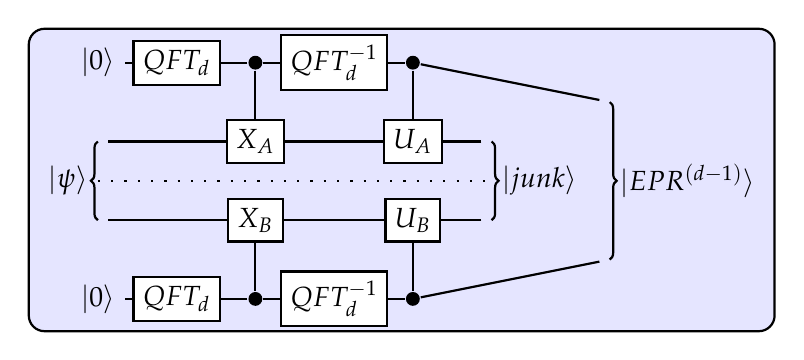
\begin{tikzpicture}[thick]
        %
        % `operator' will only be used by Hadamard (H) gates here.
        % `phase' is used for controlled phase gates (dots).
        % `surround' is used for the background box.
        \tikzstyle{operator} = [draw,fill=white,minimum size=1.5em] 
        \tikzstyle{phase} = [fill,shape=circle,minimum size=5pt,inner sep=0pt]
        \tikzstyle{surround} = [fill=blue!10,thick,draw=black,rounded corners=2mm]
        %
        % Bracket
        \draw[decorate,decoration={brace,mirror},thick] (0,-1) to
    	node[midway,left] (bracket1) {$\ket{\psi}$}
    	(0,-2);
        % Qubits
        \node at (0,0) (q1) {$\ket{0}$};
        \node at (0,-1) (q2) {};
        \node at (0,-2) (q3) {};
        \node at (0,-3) (q4) {$\ket{0}$};
        %
        % Column 1
        \node[operator] (op11) at (1,0) {$QFT_d$} edge [-] (q1);
        \node[operator] (op14) at (1,-3) {$QFT_d$} edge [-] (q4);
        %
        % Column 3
        \node[phase] (phase11) at (2,0) {} edge [-] (op11);
	\node[operator] (op22) at (2,-1) {$X_A$} edge [-] (q2);
	\node[operator] (op23) at (2, -2) {$X_B$} edge[-] (q3);
        \node[phase] (phase14) at (2,-3) {} edge [-] (op14);
        \draw[-] (phase11) -- (op22);
        \draw[-] (phase14) -- (op23);
        %
        % Column 4
        \node[operator] (op31) at (3,0) {$QFT_d^{-1}$} edge [-] (phase11);
        \node[operator] (op34) at (3,-3) {$QFT_d^{-1}$} edge [-] (phase14);
        %
        % Column 5
        \node[phase] (phase21) at (4,0) {} edge [-] (op31);
	\node[operator] (op42) at (4,-1) {$U_A$} edge [-] (op22);
	\node[operator] (op43) at (4, -2) {$U_B$} edge[-] (op23);
        \node[phase] (phase24) at (4,-3) {} edge [-] (op34);
        \draw[-] (phase21) -- (op42);
        \draw[-] (phase24) -- (op43);
        %
        % Column 6
        \node (end2) at (5,-1) {} edge [-] (op42);
        \node (end3) at (5,-2) {} edge [-] (op43);
        %
        % Bracket
        \draw[decorate,decoration={brace},thick] (5,-1) to
    	node[midway,right] (bracket) {$\ket{junk}$}
    	(5,-2);
        %
        % Column 7
        \node (end1) at (6.5,-0.5) {} edge [-] (phase21);
        \node (end4) at (6.5,-2.5) {} edge [-] (phase24);
        % Dashed line
        \draw[loosely dotted] (0,-1.5) -- (5,-1.5);
        % Bracket
        \draw[decorate,decoration={brace},thick,] (6.5,-0.5) to
    	node[midway,right] (bracket2) {$\ket{\EPR{d-1}}$}
    	(6.5,-2.5);
        %
        % Background Box
        \begin{pgfonlayer}{background} 
        \node[surround] (background) [fit = (q1) (op14) (bracket1)(bracket2)] {};
        \end{pgfonlayer}
        %
        \end{tikzpicture}
	\caption{The isometries $\Phi_A$ and $\Phi_B$.}
\end{figure}
The isometry maps the state $\ket{\psi}$ in the following steps:
\begin{enumerate}
	\item Append $\ket{0}_A$ on Alice's side and $\ket{0}_B$ on Bob's side as control registers, and
	the state becomes $\ket{\psi} \ket{0}_A \ket{0}_B$;
	\item Apply $QFT_d$ to the control registers, and the state becomes
	\begin{align}
		\frac{1}{d} \sum_{k_1,k_2 =0}^{d-1} \ket{\psi} \ket{k_1}_A \ket{k_2}_B;
	\end{align}
	\item Apply $X_A^{k_1}$ to Alice's share of $\ket{\psi}$ and $X_B^{k_2}$ to Bob's share controlled
	by the control registers, and the state becomes
	\begin{align}
		&\frac{1}{d} \sum_{k_1,k_2 =0}^{d-1}X_A^{k_1} X_B^{k_2}\ket{\psi} \ket{k_1}_A \ket{k_2}_B\\
		=&\frac{1}{d} \sum_{k_1,k_2 =0}^{d-1} \sum_{i=1}^{d-1}\sum_{j=1}^m c_j X_A^{k_1}\ket{x_{i,j}}_A X_B^{k_2}\ket{x_{i,j}}_B
		\ket{k_1}_A \ket{k_2}_B\\
		=&\frac{1}{d} \sum_{k_1,k_2 =0}^{d-1} \sum_{i=1}^{d-1}\sum_{j=1}^m c_j \omega_d^{k_1i+k_2i} \ket{x_{i,j}}_A\ket{x_{i,j}}_B
		\ket{k_1}_A \ket{k_2}_B;
	\end{align}
	\item Apply $QFT_d^{-1}$ to the control registers, and the state becomes
	\begin{align}
		&\frac{1}{d^2} \sum_{l_1,l_2 =0}^{d-1}\sum_{i=1}^{d-1}\sum_{j=1}^m c_j \omega_d^{k_1(i-l_1)+k_2(i-l_2)} \ket{x_{i,j}}_A\ket{x_{i,j}}_B
		\ket{l_1}_A \ket{l_2}_B\\
		=& \sum_{i=1}^{d-1}\sum_{j=1}^m c_j \ket{x_{i,j}}_A\ket{x_{i,j}}_B \ket{i}_A \ket{i}_B;
	\end{align}
	\item Let $n_i$ satisfy the condition $r^{n_i} \equiv i \pmod{d}$, apply $U_A^{(i)} = U_A^{n_i}$ to Alice's share of $\ket{\psi}$ and $U_B^{(i)} = U_B^{n_i}$ to Bob's share controlled
	by the control registers, and the state becomes
	\begin{align}
		&\sum_{i=1}^{d-1}\sum_{j=1}^m c_j U_A^{(i)}\ket{x_{i,j}}_A U_B^{(i)}\ket{x_{i,j}}_B \ket{i}_A\ket{i}_B \\
		=&\sum_{i=1}^{d-1} \sum_{j=1}^m c_j \ket{x_{i r^{-n_i} ,j}}_A \ket{x_{i r^{-n_i},j}}_B \ket{i}_A\ket{i}_B\\
		=& \sum_{i=1}^{d-1} \sum_{j=1}^m c_j \ket{x_{i i^{-1},j}}_A \ket{x_{i i^{-1},j}}_B \ket{i}_A\ket{i}_B\\
		= &\left(\sum_{j=1}^m c_j \ket{x_{1,j}}_A \ket{x_{1,j}}_B\right) \x \sum_{i=1}^{d-1} \ket{i}_A\ket{i}_B\\
		=&\sqrt{d-1} \left(\sum_{j=1}^m c_j \ket{x_{1,j}}_A \ket{x_{1,j}}_B\right) \x 
		\frac{1}{\sqrt{d-1}}\sum_{i=1}^{d-1}\ket{i}_A\ket{i}_B\\
		=&\sqrt{d-1} \left(\sum_{j=1}^m c_j \ket{x_{1,j}}_A \ket{x_{1,j}}_B\right) \x \ket{\EPR{d-1}},
	\end{align}
	where in the last line we used the fact that $\norm{\sum_{j=1}^m c_j \ket{x_{1,j}}_A \ket{x_{1,j}}_B} = 1/\sqrt{d-1}$.
\end{enumerate}

If the initial state is $X_A\ket{\psi}$, the isometry maps the state as following
\begin{align}
	X_A\ket{\psi} \to &X_A\ket{\psi}\ket{0}_A\ket{0}_B\\
	\to &\frac{1}{d} \sum_{k_1,k_2 =0}^{d-1} X_A\ket{\psi} \ket{k_1}_A \ket{k_2}_B \\
	\to &\frac{1}{d} \sum_{k_1,k_2 =0}^{d-1} X_A^{k_1+1} X_B^{k_2}\ket{\psi} \ket{k_1}_A \ket{k_2}_B \\
	=&\frac{1}{d} \sum_{k_1,k_2 =0}^{d-1} \sum_{i=1}^{d-1}\sum_{j=1}^m c_j \omega_d^i\omega_d^{(k_1+k_2)i} \ket{x_{i,j}}_A\ket{x_{i,j}}_B
		\ket{k_1}_A \ket{k_2}_B\\
	\to &\frac{1}{d^2}\sum_{k_1,k_2 =0}^{d-1} \sum_{i=1}^{d-1}\sum_{j=1}^m c_j \omega_d^i\omega_d^{(k_1-l_1)i+(k_2-l_2)i} \ket{x_{i,j}}_A\ket{x_{i,j}}_B
		\ket{l_1}_A \ket{l_2}_B\\
	=&\sum_{i=1}^{d-1}\sum_{j=1}^m c_j \omega_d^i \ket{x_{i,j}}_A\ket{x_{i,j}}_B \ket{i}_A \ket{i}_B\\
	\to& \sum_{i=1}^{d-1}\sum_{j=1}^m c_j \omega_d^i U_A^{(i)}\ket{x_{i,j}}_A U_B^{(i)}\ket{x_{i,j}}_B \ket{i}_A\ket{i}_B\\
	=&\sum_{i=1}^{d-1}\sum_{j=1}^m c_j \omega_d^i \ket{x_{1,j}}_A \ket{x_{1,j}}_B \ket{i}_A\ket{i}_B\\
	=&\sqrt{d-1} \left(\sum_{j=1}^m c_j \ket{x_{1,j}}_A \ket{x_{1,j}}_B\right) \x 
		\frac{1}{\sqrt{d-1}} \sum_{i=1}^{d-1}\omega_d^i \ket{i}_A\ket{i}_B\\
	=& \sqrt{d-1} \left(\sum_{j=1}^m c_j \ket{x_{1,j}}_A \ket{x_{1,j}}_B\right) \x \tX_A \ket{\EPR{d-1}},
\end{align}
where $\tX_A$ is the ideal $X$ operator.
The case of $X_B\ket{\psi}$ is similar, so we omit it here. 

If the initial state is $U_A\ket{\psi}$, the isometry maps the state as following
\begin{align}
	U_A\ket{\psi} \to &U_A\ket{\psi}\ket{0}_A\ket{0}_B\\
	\to &\frac{1}{d} \sum_{k_1,k_2 =0}^{d-1} U_A\ket{\psi} \ket{k_1}_A \ket{k_2}_B \\
	= &\frac{1}{d} \sum_{k_1,k_2=0}^{d-1} \sum_{i=1}^{d-1}\sum_{j=1}^m c_j U_A\ket{x_{i,j}}_A\ket{x_{i,j}}_B
		\ket{k_1}_A \ket{k_2}_B\\
	= & \frac{1}{d} \sum_{k_1,k_2=0}^{d-1} \sum_{i=1}^{d-1}\sum_{j=1}^m c_j \ket{x_{i r^{-1} ,j}}_A\ket{x_{i,j}}_B
		\ket{k_1}_A \ket{k_2}_B\\
	\to &\frac{1}{d} \sum_{k_1,k_2 =0}^{d-1} \sum_{i=1}^{d-1}\sum_{j=1}^m c_j X_A^{k_1} \ket{x_{i r^{-1} ,j}}_A
	X_B^{k_2}\ket{x_{i,j}}_B  \ket{k_1}_A \ket{k_2}_B \\
	=&\frac{1}{d} \sum_{k_1,k_2 =0}^{d-1} \sum_{i=1}^{d-1}\sum_{j=1}^m c_j \omega_d^{k_1 i/r}\omega_d^{k_2i} \ket{x_{ir^{-1},j}}_A\ket{x_{i,j}}_B
		\ket{k_1}_A \ket{k_2}_B\\
	\to &\frac{1}{d^2}\sum_{k_1,k_2 =0}^{d-1} \sum_{i=1}^{d-1}\sum_{j=1}^m c_j \omega_d^{k_1(i/r-l_1)}\omega_d^{(k_2(i-l_2)} \ket{x_{ir^{-1},j}}_A\ket{x_{i,j}}_B
		\ket{l_1}_A \ket{l_2}_B\\
	=&\sum_{i=1}^{d-1}\sum_{j=1}^m c_j  \ket{x_{ir^{-1},j}}_A\ket{x_{i,j}}_B \ket{ir^{-1}}_A \ket{i}_B\\
	\to& \sum_{i=1}^{d-1}\sum_{j=1}^m c_j U_A^{(ir^{-1})}\ket{x_{ir^{-1},j}}_A U_B^{(i)}\ket{x_{i,j}}_B \ket{i}_A\ket{i}_B\\
	=&\sum_{i=1}^{d-1}\sum_{j=1}^m c_j \ket{x_{1,j}}_A \ket{x_{1,j}}_B \ket{ir^{-1}}_A\ket{i}_B\\
	=&\sqrt{d-1} \left(\sum_{j=1}^m c_j \ket{x_{1,j}}_A \ket{x_{1,j}}_B\right) \x 
		\frac{1}{\sqrt{d-1}} \sum_{i=1}^{d-1}\ket{ir^{-1}}_A\ket{i}_B\\
	=& \sqrt{d-1} \left(\sum_{j=1}^m c_j \ket{x_{1,j}}_A \ket{x_{1,j}}_B\right) \x \tU_A \ket{\EPR{d-1}},
\end{align}
where $\tU_A$ is the ideal $U$ operator on Alice's side.
The derivation is similar when $U_B$ is applied, so we omit it here.
\end{proof}
%The effect of $\CHSH_X$ and $\SVT_X$ is that we have a set $\{ \ket{x_i} \}_{i \in [d]} \in \supp(\rho_A)$ such that
%\begin{align}
%	X \ket{x_i} = \omega_d^i \ket{x_i}.
%\end{align}
%The other effect of $\SVT_X$ is that we know 
%\begin{align}
%	\tA_\triangle^\diamond \rho_A \tA_\triangle^\diamond = \frac{1}{d} \ketbra{x_0}{x_0} = \frac{1}{d} \tA_\triangle^\diamond.
%\end{align}
%\hl{\textbf{Question}: Can we show $\Tr(\ketbra{x_2}{x_2} \rho_A) = 1/d$?}
In summary, for any odd prime number $d$ whose primitive root is $2$,$3$ or $5$, 
\cref{prop:realize} tells us that the correlation $C(d)$ is achievable by a quantum strategy 
and \cref{thm:selftest} tells us that the correlation $C(d)$ can self-test the EPR pair of
local dimension $d-1$. Moreover, there are infinitely many prime numbers
whose primitive root is in the set $\{2,3,5\}$ \cite{murty1988},
Hence, our main result is the following theorem.
\begin{theorem}
	There exists an infinity-sized set $D$ of prime numbers such that 
	each $d \in D$ has primitive root $2$, $3$ or $5$ and there exists
	a constant-sized correlation $C(d)$ that can self-test the EPR pair of 
	local dimension $d-1$.
\end{theorem}
We remark that our proof works for any odd prime number with primitive root $r$.
However, since there is no upper-bound of $r$ for a general prime number $d$, we 
cannot claim the corresponding correlation $C(d)$ is constant-sized. On the other
hand, since $r$ is usually much smaller than $d$, our result implies a more efficient
way to test EPR pairs of prime local dimension than the one proposed in Ref.~\cite{cgs2017}.
The size of our correlation grows linearly in $r$ whereas the Coladangelo \textit{et. al.}'s
method uses correlation grows linearly in $d$.

\bibliographystyle{alphaurl}
\bibliography{quantum_correlation}
\appendix
%========================================
\section{Proof of \cref{thm:selftest} }
\label{sec:selftest}
%========================================
This proof follows the same line of argument in Appendix A of Ref.~\cite{bamps2015}.
We first find two sum-of-square decompositions of $2\sqrt{\alpha^2+1} \1 - \I_\alpha$.
The decompositions allow us to determine some key relations between Alice and Bob's observables
and their shared state, which will be used to draw the closeness conclusion.

\begin{proof}
The first step is to find a sum-of-square decomposition of 
the following Bell expression
\begin{align}
	\bar{\I}_\alpha = 2\sqrt{\alpha^2+1} \1 - \I_\alpha
	= \frac{2}{\sin(\mu)} \1 - \frac{\cos(\mu)}{\sin(\mu)}(A_1B_1+A_1B_2) -  A_2B_1 + A_2B_2.
\end{align} 
With the following notation
\begin{align*}
	Z_A = A_1 &\quad X_A = A_2\\
	Z_B = \frac{B_1+B_2}{2\cos(\mu)} &\quad X_B = \frac{B_1-B_2}{2\sin(\mu)},
\end{align*}
the two SOS decompositions that we use are
\begin{align}
	\label{eq:sos1}&\bar{\I}_\alpha = \frac{\sin(\mu)\bar{\I}_\alpha^2 + 4\sin(\mu)\cos(\mu)^2(Z_AX_B+X_AZ_B)^2}{4},\\
	\label{eq:sos2}&\bar{\I}_\alpha = \frac{\cos^2(\mu)}{\sin(\mu)}(Z_A-Z_B)^2 + \sin(\mu) (X_A-X_B)^2.
\end{align}
The verification is omitted here.

Suppose the quantum strategy $(\ket{\psi}, \{\tilde{A}_x\}_{x=1,2}, \{\tilde{B}_{y }\}_{y=1,2}$ achieves that 
$\bra{\psi} \bar{\I}_\alpha \ket{\psi} \leq \epsilon$ where
$\bar{\I}_\alpha$ is expressed with $\tA_x$ and $\tB_y$.
The second step is to establish bounds of the following form
\begin{align}
	\label{eq:zazb} &\|(\tilde{Z}_A-\tilde{Z}_B)\ket{\psi}\| \leq c_1 \sqrt{\epsilon}\\
	\label{eq:xzxz}&\|(\tilde{X}_A(\1+\tilde{Z}_B)-\tilde{X}_B(\1-\tilde{Z}_A))\ket{\psi}\| \leq c_2 \sqrt{\epsilon}\\
	\label{eq:xaxb}&\|(\tilde{X}_A-\tilde{X}_B)\ket{\psi}\| \leq c_3 \sqrt{\epsilon}\\
	\label{eq:anticom} &\|(\tilde{Z}_A\tilde{X}_A+\tilde{X}_A\tilde{Z}_A)\ket{\psi}\| \leq c_4 \sqrt{\epsilon}.
\end{align}
Going back to the sum-of-square decomposition, we write $s = \sin(\mu)$, $c = \cos(\mu)$ and define
\begin{align*}
	S_1 = \frac{\sqrt{s}}{2} \bar{\I}_\alpha, &&
	S_2 = \sqrt{s}c(\tilde{Z}_A\tilde{X}_B+\tilde{X}_A\tilde{Z}_B),\\
	S_3 = \frac{c}{\sqrt{s}}(\tilde{Z}_A-\tilde{Z}_B), &&
	S_4 = \sqrt{s}(\tilde{X}_A-\tilde{X}_B)
\end{align*}
then 
\begin{align}
\bar{\I}_\alpha = S_1^2 + S_2^2 = S_3^2 + S_4^2
\end{align}
 and $\bra{\psi}\bar{\I}_\alpha \ket{\psi} \leq \epsilon$ implies that 
$\bra{\psi}S^2_i \ket{\psi} \leq \epsilon$ and $\|S_i \ket{\psi} \| \leq \sqrt{\epsilon}$ for $i = 1,2,3,4$.
The coefficients $c_1$, $c_2$ and $c_3$ in \cref{eq:zazb,eq:xzxz,eq:xaxb} can be determined from $S_1$,$S_2$ and $S_3$ as
\begin{align*}
	c_1 = \frac{\sqrt{s}}{c}, \quad
	c_2 = \frac{1}{\sqrt{s}} + \frac{1}{c\sqrt{s}}, \quad
	c_3 = \frac{1}{\sqrt{s}}.
\end{align*}
where we use the relation that $\tilde{X}_A(\1+\tilde{Z}_B)-\tilde{X}_B(\1-\tilde{Z}_A) = S_4/s^{1/2} + S_2/(cs^{1/2})$.
To calculate $c_4$, we use the relation
\begin{align}
	\tilde{Z}_A\tilde{X}_A + \tilde{X}_A\tilde{Z}_A = \frac{S_2}{c\sqrt{s}} + \frac{\sqrt{s}\tilde{X}_AS_3}{c} + \frac{\tilde{Z}_AS_4}{\sqrt{s}}
\end{align}
and reach the conclusion that  
\begin{align}
	c_4 = \frac{1+c+s}{c\sqrt{s}}
\end{align}
where we use that fact that $\tilde{Z}_A, \tilde{X}_A$ are unitaries.

Now we introduce the isometries $\Phi_A$ and $\Phi_B$ mentioned in the statement of the theorem.
They are the same as the ones used in Ref.~\cite{bamps2015}.
To construct $\Phi_A$ and $\Phi_B$ we need to regularize $\tZ_B$ and $\tX_B$ to make sure the corresponding operations 
are unitaries in the isometries. We define $\tZ_B^\ast$ to be the operator obtained from $\tZ_B$ by changing all the $0$-eigenvalues
to $1$ and 
\begin{align*}
\tZ_B' = \tZ_B^\ast |\tZ_B|^{-1}.
\end{align*}
In a similar way, we define $\tX_B^\ast$ and $\tX_B'$.
On Alice's side, since $\tZ_A$ and $\tX_A$ are unitaries already,
we define
\begin{align}
	\tZ_A' = \tZ_A, && \tX_A' = \tX_A.
\end{align}
The isometries are illustrated in the figure below.
\begin{figure}[H]
\center
        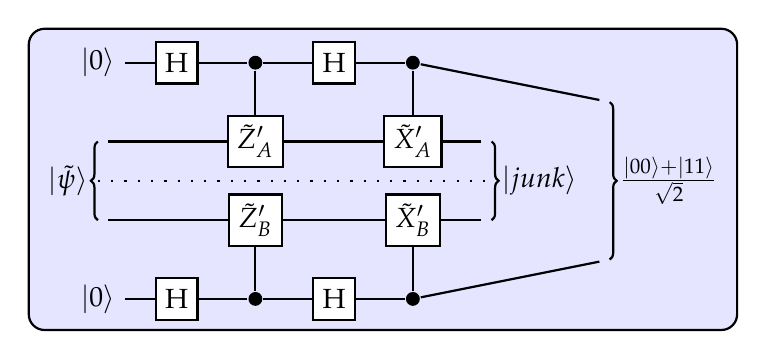
\begin{tikzpicture}[thick]
        %
        % `operator' will only be used by Hadamard (H) gates here.
        % `phase' is used for controlled phase gates (dots).
        % `surround' is used for the background box.
        \tikzstyle{operator} = [draw,fill=white,minimum size=1.5em] 
        \tikzstyle{phase} = [fill,shape=circle,minimum size=5pt,inner sep=0pt]
        \tikzstyle{surround} = [fill=blue!10,thick,draw=black,rounded corners=2mm]
        %
        % Bracket
        \draw[decorate,decoration={brace,mirror},thick] (0,-1) to
    	node[midway,left] (bracket1) {$\ket{\tpsi}$}
    	(0,-2);
        % Qubits
        \node at (0,0) (q1) {$\ket{0}$};
        \node at (0,-1) (q2) {};
        \node at (0,-2) (q3) {};
        \node at (0,-3) (q4) {$\ket{0}$};
        %
        % Column 1
        \node[operator] (op11) at (1,0) {H} edge [-] (q1);
        \node[operator] (op14) at (1,-3) {H} edge [-] (q4);
        %
        % Column 3
        \node[phase] (phase11) at (2,0) {} edge [-] (op11);
	\node[operator] (op22) at (2,-1) {$\tZ_A'$} edge [-] (q2);
	\node[operator] (op23) at (2, -2) {$\tZ_B'$} edge[-] (q3);
        \node[phase] (phase14) at (2,-3) {} edge [-] (op14);
        \draw[-] (phase11) -- (op22);
        \draw[-] (phase14) -- (op23);
        %
        % Column 4
        \node[operator] (op31) at (3,0) {H} edge [-] (phase11);
        \node[operator] (op34) at (3,-3) {H} edge [-] (phase14);
        %
        % Column 5
        \node[phase] (phase21) at (4,0) {} edge [-] (op31);
	\node[operator] (op42) at (4,-1) {$\tX_A'$} edge [-] (op22);
	\node[operator] (op43) at (4, -2) {$\tX_B'$} edge[-] (op23);
        \node[phase] (phase24) at (4,-3) {} edge [-] (op34);
        \draw[-] (phase21) -- (op42);
        \draw[-] (phase24) -- (op43);
        %
        % Column 6
        \node (end2) at (5,-1) {} edge [-] (op42);
        \node (end3) at (5,-2) {} edge [-] (op43);
        %
        % Bracket
        \draw[decorate,decoration={brace},thick] (5,-1) to
    	node[midway,right] (bracket) {$\ket{junk}$}
    	(5,-2);
        %
        % Column 7
        \node (end1) at (6.5,-0.5) {} edge [-] (phase21);
        \node (end4) at (6.5,-2.5) {} edge [-] (phase24);
        % Dashed line
        \draw[loosely dotted] (0,-1.5) -- (5,-1.5);
        % Bracket
        \draw[decorate,decoration={brace},thick,] (6.5,-0.5) to
    	node[midway,right] (bracket2) {$\frac{\ket{00}+\ket{11}}{\sqrt{2}}$}
    	(6.5,-2.5);
        %
        % Background Box
        \begin{pgfonlayer}{background} 
        \node[surround] (background) [fit = (q1) (op14) (bracket1)(bracket2)] {};
        \end{pgfonlayer}
        %
        \end{tikzpicture}
	\caption{The isometries $\Phi_A$ and $\Phi_B$.}
\end{figure}
To bound $e_{xy} := \norm{ (\Phi_A\x\Phi_B) (\tA_x \x \tB_y) \ket{\tpsi} - \ket{junk} \x (A_x\x B_y) \ket{\EPR{2}}}$,
there are some intermediate steps. Since the derivations are the same as in Ref.~\cite{bamps2015}, 
we only record the key relations here.
\begin{align}
	&\norm{(\tZ_B' - \tZ_B) \ket{\tpsi}} \leq c_1 \sqrt{\epsilon},\\
	&\norm{(\tZ_B' - \tZ_A') \ket{\tpsi}} \leq 2c_1 \sqrt{\epsilon}, \\
	&\norm{(\tX_B' - \tX_B) \ket{\tpsi}} \leq \frac{c+1}{s^{3/2}} \sqrt{\epsilon} := c_5\sqrt{\epsilon},\\
	&\norm{(\tX_B'\tZ_B'+ \tZ_B'\tX_B')\ket{\tpsi}} \leq [2c_1 + 2c_3 + 2c_5 + (\sqrt{2}+1/c)(2c_1+c_4)]\sqrt{\epsilon}
	:= c_6 \sqrt{\epsilon}.
\end{align}
Then we can calculate that 
\begin{align}
	&e_{00} = e_{10} = 2c_6 \sqrt{\epsilon}\\
	&e_{20} = 2(c_4 + c_6) \sqrt{\epsilon}\\
	&e_{01} = e_{02} = e_{11} = e_{12} = [c(c_1)+s(2c_4 + c_5) + 2c_6]\sqrt{\epsilon}\\
	&e_{21} = e_{22} = [2c_4 + c(c_1)+s(2c_4 + c_5) + 2c_6]\sqrt{\epsilon},
\end{align}
so an upper bound of the error is that
\begin{align}
	\forall x,y \in \{0,1,2\}, e_{xy} \in O((\frac{1}{cs^{1/2}} + \frac{1}{s^{3/2}})\sqrt{\epsilon}).
\end{align}
The dependence of the error term on $\alpha$ comes from the fact that 
\begin{align}
&\frac{1}{\cos(\arctan(1/\alpha)) \sin^{1/2}(\arctan(1/\alpha))} = \frac{1}{\alpha}+\frac{3}{4}\alpha - O(\alpha^3),\\
&\frac{1}{\sin^{3/2}(\arctan(1/\alpha))} = 1 + \frac{3}{4}\alpha^2 - O(\alpha^4).
\end{align}
\end{proof}
%%=====================================
\section{Equations to embed $uxu^{-1} = x^2$}
\label{sec:power2}
%%=====================================
We have order-$2$ generators $\{x_i, w_i, y_i, j_i\}_{i=1}^{7} \cup \{f\} \cup \{g_{I_i}\}_{i=1}^5$,
where each $I_i$ represent a tuple of the form $(i,j,k)$ and it means that $x_ix_jx_i = x_k$.
We have 
\begin{align}
	I_1 = (1,2,5), 
	&&I_2 = (3,5,7), 
	&&I_3 = (4,1,7), 
	&&I_4 = (4,2,6), 
	&&I_5 = (3,2,6)
\end{align} 
and we denote $C = \{I_i\}_{i=1}^5$.
The linear relations involving the generators listed above are
\begin{align}
	\label{eq:xyz} &x_i y_i z_i = e  &&\text{for} \quad i =1\dots 7 \\
	\label{eq:xfw} &x_i f w_i = e   &&\text{for} \quad i =1\dots 7 \\
	&g_{I_1} y_2z_5 =e \\
	&g_{I_2} y_5z_7 =e \\
	&g_{I_3} y_1z_7 =e \\
	&g_{I_4} y_2z_6 =e \\
	&g_{I_5} y_2z_6 =e 
\end{align}

For $j =1 \dots 7$ we introduce a set of order-$2$ generators 
$\{ y_{F_j,k}\}_{k=1}^6$ and
a group of linear relations of the form
\begin{align}
	f y_{F_j,1} y _{F_j,2} = e, && f y_{F_j,5} y_{F_j,6} = e \\
	y_j y_{F_j,2} y _{F_j,3} = e, && z_j y_{F_j,6} y_{F_j,7} = e \\
	y_{F_j,1} y_{F_j,4} y _{F_j,7} = e, && y_{F_j,3} y_{F_j,4} y_{F_j,5} = e.
\end{align}
We refer to each group of linear relations of the from above as $(F_j)$.

In the end, for each $K \in C$, 
we introduce a set of order-$2$ generators $\{y_{K,k}\}_{k=1}^6$ and
linear relations.
Suppose $K = (k_1,k_2,k_3)$, then the group of linear relations are
\begin{align}
	w_{k_1} y_{K,1} y _{K,2} = e, && w_{k_1} y_{K,5} y_{K,6} = e \\
	y_{k_2} y_{K,2} y _{K,3} = e, && z_{k_3} y_{K,6} y_{K,7} = e \\
	y_{K,1} y_{K,4} y _{K,7} = e, && y_{K,3} y_{K,4} y_{K,5} = e,
\end{align}
We refer to each group of linear relations as $(K)$.
In summary, we have $108$ binary generators, which are
\begin{align}
\{x_i, w_i, y_i, j_i\}_{i=1}^{7} \cup \{f\} \cup \{g_{I_i}\}_{i=1}^5\cup\{\{y_{F_j,k}\}_{k=1}^6\}_{j=1}^7
\cup \{\{y_{K,k}\}_{k=1}^6\}_{K \in C}.
\end{align}
In total, there are $91$ linear relations.
Converting a linear relation to a linear equation is trivial, so we omit it here.

From the group of linear relations $(F_j)$, we can deduce that for $j = 1 \dots 7$
\begin{align}
	f y_j f =& (y_{F_j,1} y _{F_j,2})(y_{F_j,2} y _{F_j,3})(y_{F_j,5} y_{F_j,6}) \\
	=&y_{F_j,1} (y_{F_j,3} y_{F_j,5}) y_{F_j,6} \\
	=& (y_{F_j,1} y_{F_j,4}) y_{F_j,6} \\
	=& y_{F_j,7} y_{F_j,6}\\
	=&z_j.
\end{align}
The immediate implication of the group of linear relations $(K)$ is that 
\begin{align}
	w_{k_1} y_{k_2} w_{k_1} =& (y_{K,1} y _{K,2})(y_{K,2} y _{K,3})(y_{K,5} y_{K,6}) \\
	=&y_{K,1} (y_{K,3} y_{K,5}) y_{K,6} \\
	=& (y_{K,1} y_{K,4}) y_{K,6} \\
	=& y_{K,7} y_{K,6}\\
	=&z_{k_3}.
\end{align}
From the conjugacy relation above, we can first deduce that 
\begin{align}
	w_{k_1}z_{k_2}w_{k_1} = w_{k_1}(f y_{k_2} f) w_{k_1} = f(w_{k_1}y_{k_2}w_{k_1}) f = fz_{k_3}f = y_{k_3}
\end{align}
where we use the fact that $(fw_{k_1})^2 = x_{k_1}^2 = e$ from \cref{eq:xfw}.
Then we can reason the relation between $x_{k_1}$, $x_{k_2}$ and $x_{k_3}$ as
follows
\begin{align}
	x_{k_1}x_{k_2}x_{k_1} = fw_{k_1}y_{k_2}z_{k_2}fw_{k_1} = (fw_{k_1}y_{k_2}w_{k_1}f)(fw_{k_1}z_{k_2}w_{k_1}f)
	=(fz_{k_3}f)(fy_{k_3}f) = y_{k_3}z_{k_3} = x_{k_3},
\end{align}
where we repeated use \cref{eq:xyz} and \cref{eq:xfw}.
In the end, we show why $I_1$,$I_2$,$I_3$,$I_4$ and $I_5$ imply that 
\begin{align}
	x_3 x_4 x_1x_2 x_4 x_3 =& x_3 (x_4 x_1x_4) (x_4x_2 x_4) x_3 \\
	=& (x_3 x_7 x_3) (x_3 x_6 x_3)\\
	=& x_5 x_2\\
	=& x_1x_2x_1 x_2
\end{align}
where we used the fact that $x_i$'s are of order-$2$.
If we treat $x_3x_4$ as $u$ and $x_1x_2$ as $x$, then we have derived that $uxu^{-1} = x^2$.



%%=====================================
\section{Equations to embed $uxu^{-1} = x^3$}
\label{sec:power3}
%%=====================================
We have order-$2$ generators $\{x_i, w_i, y_i, j_i\}_{i=1}^{8} \cup \{f\} \cup \{g_{I_i}\}_{i=1}^6$,
where each $I_i$ represent a tuple of the form $(i,j,k)$ and it means that $x_ix_jx_i = x_k$.
We have 
\begin{align*}
	&I_1 = (2,1,5), 
	&&I_2 = (1,3,6), 
	&&I_3 = (4,2,7), \\
	&I_4 = (3,2,7), 
	&&I_5 = (4,1,8),
	&&I_6 = (3,6,8)
\end{align*}
and we collect them in a set $C = \{ I_i \}_{i=1}^6$. 
The linear relations involving the generators listed above are
\begin{align}
	\label{eq:xyz} &x_i y_i z_i = e  &&\text{for} \quad i =1\dots 8 \\
	\label{eq:xfw} &x_i f w_i = e   &&\text{for} \quad i =1\dots 8 \\
	&g_{I_1} y_1z_5 =e \\
	&g_{I_2} y_3z_6 =e \\
	&g_{I_3} y_2z_7 =e \\
	&g_{I_4} y_2z_7 =e \\
	&g_{I_5} y_1z_8 =e \\
	&g_{I_6} y_6z_8 = e
\end{align}

To introduce the following linear relations, we introduce another set of 
generators $\{\{y_{F_j,k}\}_{k=1}^6\}_{j=1}^8$.
For $j =1 \dots 8$ we have a group of linear relations of the form
\begin{align}
	f y_{F_j,1} y _{F_j,2} = e, && f y_{F_j,5} y_{F_j,6} = e \\
	y_j y_{F_j,2} y _{F_j,3} = e, && z_j y_{F_j,6} y_{F_j,7} = e \\
	y_{F_j,1} y_{F_j,4} y _{F_j,7} = e, && y_{F_j,3} y_{F_j,4} y_{F_j,5} = e,
\end{align}
We refer to each group of linear relations of the from above as $(F_j)$.

The last set of linear relations comes from each $K \in C$, 
so we introduce another set of generators $\{\{y_{K,k}\}_{k=1}^6\}_{K \in C}$.
We have a group of linear relations for each $K \in C$.
Suppose $K = (k_1,k_2,k_3)$, then the group of linear relations are
\begin{align}
	w_{k_1} y_{K,1} y _{K,2} = e, && w_{k_1} y_{K,5} y_{K,6} = e \\
	y_{k_2} y_{K,2} y _{K,3} = e, && z_{k_3} y_{K,6} y_{K,7} = e \\
	y_{K,1} y_{K,4} y _{K,7} = e, && y_{K,3} y_{K,4} y_{K,5} = e,
\end{align}
We refer to each group of linear relations as $(K)$.
In summary, we have $123$ binary generators, which are
\begin{align}
\{x_i, w_i, y_i, j_i\}_{i=1}^{8} \cup \{f\} \cup \{g_{I_i}\}_{i=1}^6\cup\{\{y_{F_j,k}\}_{k=1}^6\}_{j=1}^8
\cup \{\{y_{K,k}\}_{k=1}^6\}_{K \in C}.
\end{align}
There are $106$ linear relations.
Converting a linear relation to a linear equation is trivial, so we omit it here.

The derivation of $fy_jf=z_j$ from the group of linear relations $(F_j)$for $j = 1 \dots 8$
is the same as the previous case, so we omit it here.
We also omit the derivation of $x_{k_1} x_{k_2} x_{k_1} = x_{k_3}$, 
from the group of linear relations $(K)$,
for each $K \in C$.
In the end, we show the implication of the conjugacy relations in $C$ as follows 
\begin{align*}
	x_3 x_4 x_1x_2 x_4 x_3 =& x_3 (x_4 x_1x_4) (x_4x_2 x_4) x_3 \\
	=& (x_3 x_8 x_3) (x_3 x_7 x_3)\\
	=& x_6 x_2\\
	=& x_1x_5x_1 x_2\\
	=&x_1x_2x_1x_2x_1x_2
\end{align*}
where we used the fact that $x_i$'s are of order-$2$.
If we treat $x_3x_4$ as $u$ and $x_1x_2$ as $x$, then we have derived that $uxu^{-1} = x^3$.



%%=====================================
\section{Equations to embed $uxu^{-1} = x^5$}
\label{sec:power5}
%%=====================================
We have order-$2$ generators $\{x_i, w_i, y_i, j_i\}_{i=1}^{10} \cup \{f\} \cup \{g_{I_i}\}_{i=1}^8$,
where each $I_i$ represent a tuple of the form $(i,j,k)$ and it means that $x_ix_jx_i = x_k$.
We have 
\begin{align*}
	&I_1 = (2,1,5), 
	&&I_2 = (1,3,6), 
	&&I_3 = (2,6,7), 
	&&I_4 = (1,7,8), \\
	&I_5 = (4,1,9),
	&&I_6 = (3,8,9),
	&&I_7 = (4,2,10)
	&&I_8 = (3,2,10)
\end{align*}
and we collect them in a set $C = \{ I_i \}_{i=1}^8$. 
The linear relations involving the generators listed above are
\begin{align}
	\label{eq:xyz} &x_i y_i z_i = e  &&\text{for} \quad i =1\dots 10 \\
	\label{eq:xfw} &x_i f w_i = e   &&\text{for} \quad i =1\dots 10 \\
	&g_{I_1} y_1z_5 =e \\
	&g_{I_2} y_3z_6 =e \\
	&g_{I_3} y_6z_7 =e \\
	&g_{I_4} y_7z_8 =e \\
	&g_{I_5} y_1z_9 =e \\
	&g_{I_6} y_8z_9 = e\\
	&g_{I_7} y_2z_{10} =e \\
	&g_{I_8} y_2z_{10} = e
\end{align}

To introduce the following linear relations, we introduce another set of 
generators $\{\{y_{F_j,k}\}_{k=1}^6\}_{j=1}^{10}$.
For $j =1 \dots 10$ we have a group of linear relations of the form
\begin{align}
	f y_{F_j,1} y _{F_j,2} = e, && f y_{F_j,5} y_{F_j,6} = e \\
	y_j y_{F_j,2} y _{F_j,3} = e, && z_j y_{F_j,6} y_{F_j,7} = e \\
	y_{F_j,1} y_{F_j,4} y _{F_j,7} = e, && y_{F_j,3} y_{F_j,4} y_{F_j,5} = e,
\end{align}
We refer to each group of linear relations of the from above as $(F_j)$.

The last set of linear relations comes from each $K \in C$, 
so we introduce another set of generators $\{\{y_{K,k}\}_{k=1}^6\}_{K \in C}$.
We have a group of linear relations for each $K \in C$.
Suppose $K = (k_1,k_2,k_3)$, then the group of linear relations are
\begin{align}
	w_{k_1} y_{K,1} y _{K,2} = e, && w_{k_1} y_{K,5} y_{K,6} = e \\
	y_{k_2} y_{K,2} y _{K,3} = e, && z_{k_3} y_{K,6} y_{K,7} = e \\
	y_{K,1} y_{K,4} y _{K,7} = e, && y_{K,3} y_{K,4} y_{K,5} = e,
\end{align}
We refer to each group of linear relations as $(K)$.
In summary, we have $157$ binary generators, which are
\begin{align}
\{x_i, w_i, y_i, j_i\}_{i=1}^{10} \cup \{f\} \cup \{g_{I_i}\}_{i=1}^8\cup\{\{y_{F_j,k}\}_{k=1}^6\}_{j=1}^{10}
\cup \{\{y_{K,k}\}_{k=1}^6\}_{K \in C}.
\end{align}
There are $136$ linear relations.
Converting a linear relation to a linear equation is trivial, so we omit it here.

The derivation of $fy_jf=z_j$ from the group of linear relations $(F_j)$for $j = 1 \dots 10$
is the same as the previous case, so we omit it here.
We also omit the derivation of $x_{k_1} x_{k_2} x_{k_1} = x_{k_3}$, 
from the group of linear relations $(K)$,
for each $K \in C$.
In the end, we show the implication of the conjugacy relations in $C$ as follows 
\begin{align*}
	x_3 x_4 x_1x_2 x_4 x_3 =& x_3 (x_4 x_1x_4) (x_4x_2 x_4) x_3 \\
	=& (x_3 x_9 x_3) (x_3 x_{10} x_3)\\
	=& x_8 x_2\\
	=& (x_1x_7x_1) x_2\\
	=&x_1(x_2 x_6 x_2)x_1x_2\\
	=& x_1x_2(x_1x_5x_1)x_2x_1x_2\\
	=&x_1x_2x_1(x_2x_1x_2)x_1x_2x_1x_2
\end{align*}
where we used the fact that $x_i$'s are of order-$2$.
If we treat $x_3x_4$ as $u$ and $x_1x_2$ as $x$, then we have derived that $uxu^{-1} = x^5$.



\end{document}
